\documentclass[a4paper,12pt]{report}

% Definizioni
\def\titolotesi{Uso di Computer Quantistici per lo studio di sistemi elementari}
\def\laureando{Davide Pruscini}
\def\annoaccademico{2019--2020}

%Commenti
\usepackage{verbatim}
\usepackage[hyphens]{url}

\begin{comment}
File previsti in input:
	Introduzione.tex
	Capitolo1.tex
	Capitolo2.tex
	Capitolo3.tex
	Conclusioni.tex
	Bibliografia.bib
	Codice.tex
	Glossario.tex
	LinkFigure.tex
\end{comment}

% Title Page
\title{\begin{large}\textbf{\titolotesi}\end{large}}
\author{\laureando}

% Hyperlinks
\usepackage{hyperref}
\hypersetup{
    colorlinks=true,
    citecolor=black,
    linkcolor=black,     
    urlcolor=cyan,
}

% Citazioni
\usepackage{dirtytalk}

% Equazioni, Matrici ecc.
\usepackage{amsmath}
\usepackage{amsfonts}
\usepackage{siunitx}

% Righe multiple tabella
\usepackage{multirow}
\usepackage{adjustbox}

%Parole accentate
\usepackage[T1]{fontenc}
%\usepackage[utf8x]{inputenc}

%Parole di sistema in italiano (Indice, Capitolo, ...)
\usepackage[italian]{babel}

%Colori
\usepackage{xcolor}
\usepackage{url}

%Codice
\usepackage{minted}
\usepackage{listings}

%Accostare Figure e Table
\usepackage{caption}
\usepackage{subcaption}

%Impaginazione
\usepackage{fancyhdr}
\fancyhf{}
\fancyfoot[LE,RO]{\thepage}

\usepackage{epsfig}

%Numero di pagina romano
\pagenumbering{Roman}

%\usepackage{setspace}
\newlength\sinistra
\newlength\corpo
\newlength\pagina
\setlength {\pagina} {21cm}
\setlength {\sinistra} {1.46cm}
\setlength {\corpo} {13.5cm}
\textwidth \the\corpo
\hoffset \the\sinistra
\paperwidth \the\pagina
\linespread{1.6}

\begin{document}

%FRONTESPIZIO
\begin{titlepage}

\begin{center}
\textsc{\Large Università degli Studi di Perugia}\medskip\\

{\Large Dipartimento di Matematica e Informatica}\medskip\\

\rule{10mm}{0.01mm}\medskip\\

{\small \textsc{Corso di Laurea Triennale in Informatica}}\medskip\\

\vspace*{3mm}


\includegraphics[scale=0.70]{LogoUniPG.png}

\Large Tesi di Laurea \par\bigskip

{\large \bf \titolotesi \par}

\end{center}\par

\hspace{0.05cm}Laureando:\hspace{7.3cm}Relatore:\par

\hspace{0.0cm}\emph{\laureando}\hfill\emph{Prof.~Osvaldo Gervasi}
\hspace*{7cm}\ \hfill \emph{Dott. Damiano Perri}
\hspace*{7cm}\ \hfill \emph{Dott. Marco Simonetti}
\vfill

\begin{center}

\rule{40mm}{0.01mm}

Anno Accademico \annoaccademico

\end{center}

\end{titlepage}

%INDICE
%Numero di sottocapitoli da mostrare
\setcounter{tocdepth}{3}
%Numero di sottocapitoli da numerare
\setcounter{secnumdepth}{3}
\tableofcontents

%ELENCO DELLE FIGURE
\listoffigures

%ELENCO DELLE TABELLE
\listoftables

%CORPO TESI
\pagestyle{fancy}

%INTRODUZIONE
\chapter*{Introduzione}
\fancyhead[RO, LE]{\bfseries Introduzione}

\pagenumbering{arabic}
Questa tesi nasce con l'intento di analizzare l'applicazione pratica di un computer quantistico, in collaborazione con il gruppo \textit{Computational Dynamics and Kinetics} del Dipartimento di Chimica, Biologia e Biotecnologie dell'Università di Perugia, coordinato dalla Dott.ssa Noelia Faginas Lago.  In particolare si vuole misurare l'energia di legame della molecola in funzione dell'interdistanza atomica tra gli atomi costituenti.

La molecola che analizzeremo principalmente sarà l'Idrogeno ($H_2$) in quanto, grazie alla sua semplice struttura, non richiederà tempi di esecuzione troppo lunghi.

Nel raggiungere questo obbiettivo si è voluto far conoscere come con il passare del tempo, a seguito di continue ricerche e studi, si è arrivati dai computer classici attualmente utilizzati, allo studio e realizzazione di un computer quantistico. Negli ultimi quattro anni, dopo l'annuncio da parte di IBM di una linea di prodotti di computer quantistici, c'è stata una forte crescita di prodotti apparsi nel mercato e un enorme e crescente interesse su questa tematica.

È stato necessario quindi descrivere le caratteristiche di un computer quantistico, a partire dal concetto base di qubit e di porta logica quantistica, fino ad arrivare alle classi di complessità e all'algoritmo VQE, che utilizzeremo nella fase sperimentale.

Infine si descrive il framework utilizzato che ci ha permesso di simulare il comportamento di un computer quantistico per i nostri test, restituendo quindi grafici e risultati.
\addcontentsline{toc}{chapter}{Introduzione}

\begin{comment}
Tutti i capitoli dovranno iniziare con la seguente intestazione:
\chapter{Titolo capitolo}
\fancyhead[RO, LE]{\bfseries Titolo capitolo}
\end{comment}

%CAPITOLI
\chapter{Quando la legge di Moore volge al termine}
\fancyhead[RO, LE]{\bfseries Quando la legge di Moore volge al termine}
In questo capitolo si vogliono introdurre due tipologie di computer, a partire da quello moderno che tutti noi conosciamo fino ad arrivare alla nascita di quello quantistico, mettendo in evidenza l'importanza del suo sviluppo.


\section{I computer classici}
\textit{Un computer è una macchina automatizzata che svolge due operazioni fondamentali: effettua complessi calcoli matematici ed elabora informazioni; spetta quindi al programmatore impartire ordini all'elaboratore per risolvere determinate problematiche \cite{computer2004articolo}.}

Le prime informazioni e testimonianze storiche a noi note riguardanti gli algoritmi di calcolo sono molto antiche, per avere una definizione formale di algoritmo si è dovuto attendere sino agli anni '30, dove in maniera indipendente, Alonzo Church ed Alan Turing si impegnarono nella risoluzione di un problema posto da David Hilbert qualche anno prima.
La questione su cui si interrogò riguardava l'esistenza di algoritmi capaci di risolvere ogni problema della matematica, introducendo così il concetto di problema decisionale.

Fu Turing che nel 1936, dopo aver pubblicato un articolo teorico, sviluppò un modello per la computazione in grado di eseguire algoritmi, chiamato macchina di Turing \cite{turing1936articolo}.
Quest'ultimo diede poi luogo allo sviluppo dell'attuale computer moderno e successivamente dimostrò anche l'esistenza di una macchina di Turing universale, la quale poteva essere usata per simulare le operazioni svolte in una qualsiasi macchina di Turing.

Dato quindi un algoritmo eseguibile su qualsiasi hardware, esiste il suo equivalente per una macchina di Turing universale che esegue lo stesso esatto compito.
Il concetto di \say{efficienza} \cite{dipierro2013articolo} di un algoritmo ci permette di capire meglio i vantaggi della computazione quantistica, che espressa in termini matematici nella teoria della complessità computazionale può essere riassunta brevemente come segue: un algoritmo è efficiente se il tempo di esecuzione è una funzione polinomiale rispetto alla grandezza del problema risolto (o lunghezza dell'input); un algoritmo è inefficiente se il tempo di esecuzione è superiore al polinomiale (tipicamente esponenziale).

Alla fine degli anni '60 e all'inizio degli anni '70 venne introdotta la tesi di Church-Turing i quali affermavano di poter simulare efficientemente su di una macchina di Turing un qualsiasi processo algoritmico.

Con l'aumentare della potenza degli hardware in maniera esponenziale, Gordon Moore nel 1965 codificò questa crescita attraverso la legge di Moore:
\begin{center}
\textit{\say{La complessità di un microcircuito, misurata ad esempio tramite il numero di transistor per chip, raddoppia ogni 18 mesi} \cite{moore2006articolo}.}
\end{center}

La fabbricazione futura di componenti hardware sempre più piccoli, porterà all'invalidità di questa legge a causa di problemi dovuti alla dimensione fisica delle componenti: da qui nasce l'esigenza da parte del mondo scientifico di scoprire nuove tipologie di macchine che vanno oltre le limitazioni imposte dalla legge di Moore.

\subsection{La Macchina di Turing}
Possiamo definire la macchina di Turing come un insieme di componenti: un programma, un controllo a stati finiti, un nastro ed una testina di lettura/scrittura \cite{turing_machine2014articolo}.

A differenza di un semplice computer, questa macchina si basa su un modello ideale dove non sono presenti limiti di dimensioni, la sua realizzazione si approccia ad un modello a circuiti dove grazie all'utilizzo di porte sarà possibile trasportare informazioni.
\begin{figure}[htp]
    \centering
    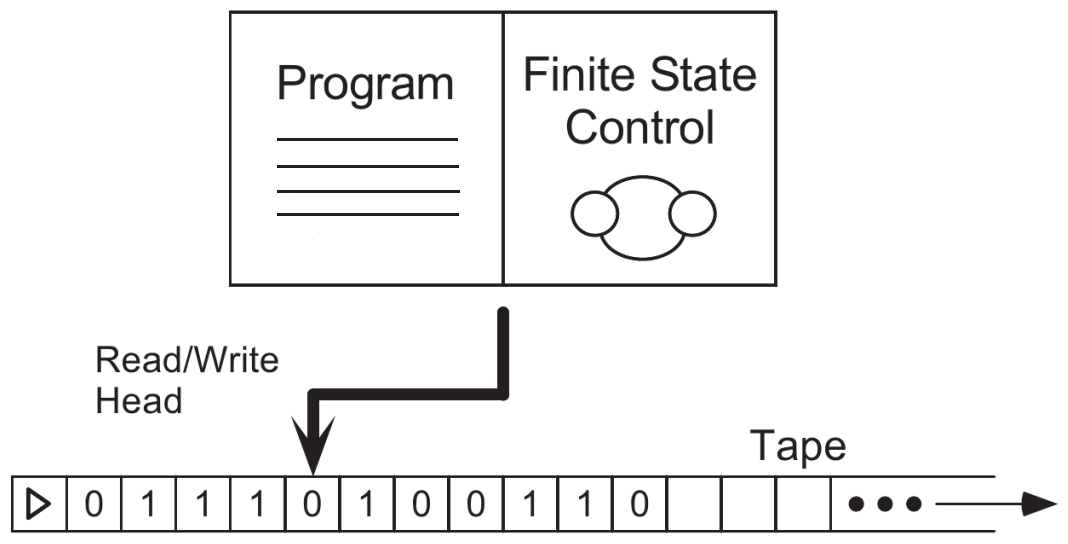
\includegraphics[width=8cm]{Images/Capitolo1/macchina_turing.png}
    \caption{Schema della Macchina di Turing.}
    \label{fig:macchina_turing}
\end{figure}
\newline
Ogni componente ha un suo scopo ben preciso: il controllo a stati finiti può essere paragonato ad un processore che può assumere un insieme finito di stati ($q_1, q_2, ..., q_m$); il nastro si può immaginare come una sequenza di caselle, ognuna delle quali conterrà un simbolo letto dalla stringa in input.

La testina può scorrere il nastro di una casella alla volta e agire su di essa di conseguenza.
Prima dell'esecuzione il controllo si troverà nello stato di partenza $q_i$ e la testina indicherà il simbolo $\rhd$ all'inizio del nastro.
Il programma, costituito da una quintupla di elementi, regola l'evoluzione dell'algoritmo.

Per prima cosa viene selezionata la stringa che ha come primo elemento lo stato in cui si trova il controllo e come secondo, il simbolo indicato dalla testina.
Se la stringa cercata non è presente nel programma la macchina assume lo stato di arresto $q_h$ e l'esecuzione del programma termina, in caso contrario la configurazione della macchina cambierà e verranno analizzati i tre elementi successivi.
Questi elementi rappresentano rispettivamente: lo stato che il controllo dovrà assumere, un simbolo di $\Gamma$ che la testina scrive sulla casella puntata e lo spostamento facoltativo della testina di una casella, a sinistra o a destra sul nastro.
Fino a quando la macchina non assume lo stato $q_h$ il ciclo prosegue, quando questo avviene l'output del programma sarà memorizzato nella casella su cui punta la testina.

La macchina di Turing che è stata presa in esame è la più semplice, altre varianti possono differire nel numero di nastri o nella loro dimensionalità, rimanendo tuttavia equivalenti.

Nella Figura \ref{fig:esempio_turing} viene mostrato un esempio di automa di macchina di Turing in grado risolvere il problema del riporto, o più semplicemente, di sommare 1 alla stringa di bit letta in input.
\newline
\begin{figure}[htp]
    \centering
    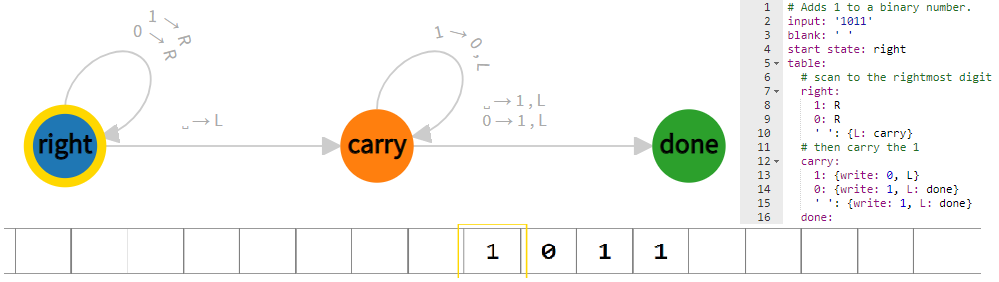
\includegraphics[width=11cm]{Images/Capitolo1/esempio_turing.png}
    \caption{Problema del riporto su Macchina di Turing.}
    \label{fig:esempio_turing}
\end{figure}

\section{I computer quantistici}
\textit{Il computer quantistico non si basa su un modello computazionale classico, utilizza piuttosto i principi della meccanica quantistica per la risoluzione di problemi che appartengono alle più svariate categorie. Tra queste troviamo la chimica quantistica e l'informatica quantistica, con tutte le loro sfaccettature \cite{hofmann2003articolo}.} 

Alla fine degli anni '70 la computazione classica probabilistica acquistò enorme importanza in ambito informatico e di conseguenza vennero implementati i primi algoritmi non deterministici, facendo così nascere dei dubbi sulla tesi di Church-Turing \cite{church1985articolo}.

Iniziò la ricerca di un modello computazionale in grado di simulare efficientemente qualsiasi altro modello computazionale.
La prima proposta di computer quantistico apparve nel 1959 grazie a Richard Feynman, in seguito, nel 1982 il fisico Paul Benioff \cite{quantum2001articolo} riuscì a dimostrare che la macchina di Turing classica poteva simulare certi fenomeni fisici senza incorrere in un rallentamento esponenziale delle sue prestazioni. Tre anni dopo David Deutsch \cite{hofmann2003articolo} ipotizzò che, essendo in definitiva le leggi della fisica approssimabili a quelle della meccanica quantistica, si potesse usare un dispositivo basato sui principi della meccanica quantistica per simulare efficientemente un sistema fisico arbitrario.

Le vere potenzialità di questa nuova scienza vennero messe in risalto nei primi anni Novanta da Richard Jozsa, il quale nel 1991, dopo aver descritto quali sono le funzioni che non possono essere risolte dal parallelismo quantistico, collaborò con Deutsch proponendo il primo problema che una macchina quantistica riusciva a risolvere in tempi più rapidi rispetto ad una deterministica.

La svolta epocale si ebbe nel 1994 con Peter Shor il quale pubblicò un algoritmo quantistico riuscendo a risolvere il problema della fattorizzazione di numeri molto grandi in un tempo polinomiale; due anni dopo Lov Grover scoprì la possibilità di trovare un record all'interno di un database in tempi più brevi rispetto agli algoritmi adottati nei computer classici \cite{algorithm2018articolo}.

Questi sviluppi portarono alla concezione odierna di computer quantistici: calcolatori che sfruttano le leggi della fisica e della meccanica quantistica con una capacità di calcolo, per alcune tipologie di problemi, di gran lunga superiore rispetto al computer classico.

Lo studio di queste macchine ha dato origine ad un nuovo settore della ricerca teorica nell'informatica e nella fisica che prende il nome di computazione quantistica, la quale stravolgerà completamente il trattamento dell'informazione, riuscendo a risolvere problemi scientifici attualmente irrisolvibili.

\subsection{Sviluppi nell'era moderna}
Tra la fine degli anni Novanta e i primi anni Duemila vennero condotti diversi esperimenti che diedero alla luce i primi computer quantistici, basati su un numero esiguo di qubit ($2\div 7$).
Questi esperimenti, effettuati nelle università di Stanford, Monaco e nel Laboratorio Nazionale di Los Alamos, riuscirono a svolgere gli algoritmi di Deutsch e Shor.

Successivamente ebbero luogo altre scoperte e furono dimostrate ulteriori teorie, mirate sia allo sviluppo della macchina quantistica sia ai campi scientifici correlati.

A seguito di questi sviluppi è stato possibile realizzare componenti fisiche fino ad ora inesistenti, in grado di contribuire alla costruzione del primo computer di questo genere e contemporaneamente vennero sperimentate le prime reti quantistiche.
La rete quantistica DARPA \cite{qnetwork2005articolo} fu una di queste e venne resa operativa nel 2003; nel 2005 gli scienziati del Max Planck Institute sono riusciti a realizzare un prototipo funzionante e nello stesso anno, venne annunciato il primo qubyte.

Nel 2007 fa la sua prima apparizione pubblica la D-Wave System, azienda che produce quello che viene considerato il primo computer quantistico adiabatico a 16qubit, definito in questo modo dato che ricorda le trasformazioni adiabatiche della termodinamica: un sistema scambia e riacquista calore per gradi e non tutto in un unico istante.
Il primo computer quantistico fu commercializzato nel 2011 e prese il nome di D-Wave One, costituito da 128qubit; insieme al suo successore D-Wave Two furono entrambi acquistati da Google in collaborazione con la NASA.

Tutto questo creò molto scalpore a livello accademico e scontri di idee: alcuni erano convinti delle sue potenzialità, mentre altri cercavano di dimostrare che non si trattava di vere e proprie macchine quantistiche, ma soltanto di macchine classiche che sfruttavano effetti quantistici per velocizzare i calcoli.

Alcune delle più grandi aziende in campo tecnologico come IBM e Google ne hanno capito l'importanza ed è per questo che puntano alla costruzione e allo sviluppo di queste macchine \cite{preskill2018articolo}.

\chapter{Computazione quantistica}
\fancyhead[RO, LE]{\bfseries Computazione quantistica}
In questo capitolo si andranno ad approfondire i concetti su cui si basa un computer quantistico, a partire dalla più piccola unità d'informazione, in contrapposizione al bit classico. Si analizzeranno alcune delle sue proprietà fino ad avere una visione d'insieme sia algebrica che geometrica, facendo particolare attenzione alle componenti necessarie per effettuare operazioni con una macchina di questo tipo.

\section{Bit e qubit}
L'unità più piccola d'informazione per i computer classici è il bit: dal punto di vista fisico è un sistema a due stati che può assumere soltanto valore 0 o 1.

Il computer quantistico invece utilizza i qubit \cite{dipierro2013articolo, cambridge2010book} (quantum bit), una particella che si sottomette alle regole della fisica quantistica esistendo in due stati nello stesso istante: potrà assumere sia 1 che 0 contemporaneamente, come mostrato in Figura \ref{fig:bit_qubit}.
\begin{figure}[htp]
    \centering
    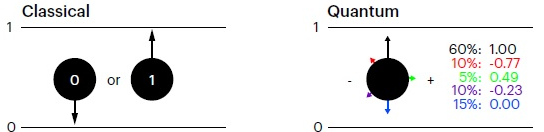
\includegraphics[width=10cm]{Images/Capitolo2/bit_qubit.png}
    \caption{Bit e qubit a confronto.}
    \label{fig:bit_qubit}
\end{figure}

Fu Benjamin Schumacher, presso il Kenyon College (Ohio), che descrisse questo sistema fisico quantistico: più semplice, versatile e potente rispetto a quello digitale.
Per capire la natura di questa entità e la differenza con la sua istanza classica, il bit, dobbiamo fare riferimento alle leggi che regolano il comportamento e l'evoluzione di un sistema fisico reale e di conseguenza l'elaborazione dell'informazione in esso contenuta.

Grazie ad alcuni postulati della meccanica quantistica è stato possibile allargare il campo d'azione di un calcolatore, osservandolo da un'altra prospettiva.
Per questo motivo lo spazio occupato dalle classiche sequenze binarie (registri di bit) includerà tutte le infinite combinazioni (principio di sovrapposizione degli stati) con le loro interazioni non classiche (fenomeno dell'interferenza), che porteranno un effetto sui risultati finali (principio di misurazione) \cite{dipierro2013articolo}.

% Entanglement = Correlazione quantistica
\subsection{Sovrapposizione e entanglement}
Facendo sempre riferimento alla fisica quantistica possiamo identificare il qubit come un vettore $\psi$ nello spazio complesso bidimensionale $\mathbb{C}^2$ (Spazio di Hilbert) definito nella forma
\begin{equation}
    |\psi\rangle = \alpha|0\rangle + \beta|1\rangle =
    \alpha
    \begin{bmatrix}
        0\\
        1
    \end{bmatrix} +
    \beta
    \begin{bmatrix}
        1\\
        0
    \end{bmatrix},
\end{equation}
dove gli scalari $\alpha$ e $\beta$ sono numeri complessi che esprimono l'ampiezza di probabilità dello stato $|0\rangle$ e $|1\rangle$, rispettivamente.
Questi stati intermedi del qubit vengono chiamati sovrapposizioni degli stati e possono essere interpretati come una coesistenza degli stessi in determinate proporzioni: la probabilità che un qubit possa essere 0 oppure 1 è del tutto priva di garanzie e si basa soltanto su situazioni di incertezza.

Esiste inoltre uno stato di correlazione tra due o più sistemi quantistici, che prende il nome di entanglement: in esso due sistemi risultano connessi in un rapporto di causa-effetto, pur non essendo a contatto diretto o indiretto.
A seguito di questo, possiamo introdurre il \say{teletrasporto quantistico} ossia la trasmissione di uno stato quantistico da un punto ad un altro con velocità istantanea \cite{cambridge2010book}.

Entrambi questi fenomeni non sono però sufficienti a fornire una lettura corretta su di un qubit dato che l'informazione trasmessa non si può ritenere certa.
La non-località è un altro principio quantistico dove si afferma che l'entanglement non dipende dalla distanza tra le particelle, le quali possono trovarsi molto lontane tra di loro.

\subsection{Rappresentazione di un qubit nella sfera di Bloch}
All'interpretazione algebrica di un qubit, precedentemente illustrata, possiamo associare anche quella geometrica che ci aiuta ad avere un'intuizione visiva di questa entità, rappresentandola sulla superficie di una sfera unitaria nello spazio reale a tre dimensioni: questa sfera prende il nome dal fisico svizzero Felix Bloch \cite{dipierro2013articolo}.
\begin{figure}[htp]
    \centering
    
\includegraphics[width=8cm]{Images/Capitolo2/sfera_bloch.png}
    \caption{Interpretazione geometrica bit e qubit.}
    \label{fig:sfera_bloch}
\end{figure}
\newline

Nella Figura \ref{fig:sfera_bloch} possiamo notare come polo nord e polo sud siano associati rispettivamente allo stato quantistico $|0\rangle$ e $|1\rangle$.
Ogni operazione svolta su di un qubit all'interno della sfera, verrà visualizzata come una rotazione all'interno di essa.
Volendo effettuare una rotazione inversa per riportare il punto nella sua posizione originale, anche il qubit può essere invertito e riportato dallo stato finale nello stato iniziale, annullando il suo effetto.

Questa caratteristica prende il nome di reversibilità computazionale e caratterizza fortemente la computazione quantistica.

\subsection{Problema della misurazione quantistica}
Prima di addentrarci nella misurazione di uno stato quantistico introduciamo il concetto di sistema coerente:
\begin{center}
\textit{Un sistema viene definito coerente se determina una fuoriuscita parziale dell'informazione contenuta al suo interno durante l'interazione con un elemento esterno, come ad esempio un misuratore.} \cite{dipierro2013articolo}
\end{center}
Prendendo in considerazione un sistema di piccole dimensioni, come ad esempio un atomo, vogliamo misurare la posizione in cui si trova un elettrone all'interno di esso.

Questo elettrone inizialmente si troverà in una posizione che chiameremo $x$, una volta inserito nel sistema il nostro misuratore possiamo sparare un fotone, così da far muovere l'elettrone che risulterà essere in una nuova posizione che chiameremo $y$.

Possiamo ricondurre questo esempio alla misurazione di un qubit all'interno della sfera di Bloch, ipotizzando di effettuare un qualche tipo di operazione su di esso non avremo modo di misurare coerentemente la sua posizione in quanto si tratta di una misurazione quantistica.
Quest'ultima per essere svolta richiederà la perturbazione del sistema il quale collasserà introducendo determinazione: se ci si trova in uno stato di sovrapposizione la misurazione che andrò a fare ricadrà su uno stato ben preciso e non sulla sovrapposizione stessa.

\section{Porte quantistiche}
I cambiamenti che si verificano in uno stato quantistico possono essere descritti usando il linguaggio del calcolo quantistico.
Come per i computer classici, costituiti da un circuito elettrico contenente fili e porte logiche, così i computer quantistici avranno un circuito quantistico contenente fili e porte quantistiche elementari, in modo da manipolare e trasportare l'informazione quantistica.

L'utilizzo di matrici per rappresentare operazioni lineari \cite{algebra2015book} su di un qubit risulta essere il modo più conveniente.

\subsection{Porte a qubit singolo}
Nei computer classici si può individuare un'unica porta logica (non banale) a un bit, la porta NOT; il cui comportamento può essere completamente descritto dalla sua tabella di verità, dalla quale si evince che l'operazione logica effettuata è quella di una negazione, dove $0\rightarrow1$ e $1\rightarrow0$.

Per definire un'operazione analoga su un qubit, non possiamo limitarci a stabilire la sua azione sugli stati di base $|0\rangle$ e $|1\rangle$, ma dobbiamo specificare anche come deve essere trasformato un qubit che si trova in una sovrapposizione degli stati $|0\rangle$ e $|1\rangle$.
Intuitivamente, il NOT dovrebbe scambiare i ruoli dei due stati fondamentali e trasformare $\alpha|0\rangle + \beta|1\rangle$ in $\alpha|1\rangle + \beta|0\rangle$.
Chiaramente $|0\rangle$ si trasformerebbe in $|1\rangle$ e $|1\rangle$ in $|0\rangle$.

La matrice corrispondente al NOT quantistico, denominata $X$, viene definita come segue:
\begin{equation}
    X=
    \begin{bmatrix}
        0 & 1\\
        1 & 0
    \end{bmatrix}
\end{equation}

L'applicazione di $X$ a un qubit $\alpha|0\rangle + \beta|1\rangle$ risulterà essere:
\begin{equation}
    X
    \begin{bmatrix}
        \alpha \\
        \beta
    \end{bmatrix} =
    \begin{bmatrix}
        \beta \\
        \alpha
    \end{bmatrix}
\end{equation}

Generalmente un'operazione su un singolo qubit può essere rappresentata da una matrice $2\times2$; bisogna però specificare che non tutte le matrici di questo tipo definiscono operazioni \say{lecite} su un qubit; per questo motivo deve essere sempre vera la seguente condizione di normalizzazione \cite{zhao2020articolo}, in qualsiasi stato quantistico esso si trovi:
\begin{equation}
    |\alpha|^2 + |\beta|^2 = 1
\end{equation}

Come abbiamo già detto precedentemente, possiamo definire una sola operazione non banale su un singolo bit, invece per quanto riguarda la computazione quantistica, esistono molte operazioni non banali che agiscono su di un qubit.

Altre due porte di notevole importanza sono la $Z$
\begin{equation}
    Z=
    \begin{bmatrix}
        1 & 0\\
        0 & -1
    \end{bmatrix}
\end{equation}
e la porta Hadamard
\begin{equation}
    H=
    \dfrac{1}{\sqrt{2}}
    \begin{bmatrix}
        1 & 1\\
        1 & -1
    \end{bmatrix}
\end{equation}

La porta $Z$ ha il compito di lasciare invariato lo stato $|0\rangle$ ed invertire il segno dello stato $|1\rangle$ mentre la porta $H$, utilizzata maggiormente, ha il compito di trasformare uno stato base in una sovrapposizione.
L'azione sullo stato $\psi$ sarà quindi definita come segue:
\small
\begin{equation}
    |\psi'\rangle = H
    \begin{bmatrix}
        \alpha\\
        \beta
    \end{bmatrix} =
    \dfrac{1}{\sqrt{2}}
    \begin{bmatrix}
        \alpha + \beta\\
        \alpha - \beta
    \end{bmatrix} =
    \dfrac{1}{\sqrt{2}}
    (\alpha + \beta)|0\rangle +
    \dfrac{1}{\sqrt{2}}
    (\alpha - \beta)|1\rangle
\end{equation}
\normalsize

Per visualizzare l'azione della porta $H$ conviene utilizzare la sfera di Bloch, come mostrato in Figura \ref{fig:hadamard_sfera_bloch}.
Questa porta è rappresentata da una rotazione attorno all'asse $y$ di \ang{90}, seguita da una rotazione attorno all'asse $x$ di \ang{180}.
La sovrapposizione che si genera, dopo una misurazione nella base computazionale, risulta essere $|0\rangle$ oppure $|1\rangle$ con uguale probabilità.
Applicando per esempio $H$ a $|0\rangle$ si ottiene:
\begin{equation}
    H|0\rangle = H
    \begin{bmatrix}
        1\\
        0
    \end{bmatrix} =
    \dfrac{1}{\sqrt{2}}
    \begin{bmatrix}
        1\\
        1
    \end{bmatrix} =
    \dfrac{1}{\sqrt{2}}
    (|0\rangle + |1\rangle)
\end{equation}

L'effetto di $H$ si può quindi vedere come un NOT eseguito a metà, in modo che lo stato risultante non è né 0 né 1, bensì una sovrapposizione dei due stati di base.
Considerando il significato puramente fisico di questa porta si può verificare che $H^2$ è l'identità e quindi applicando due volte $H$ ad uno stato quest'ultimo risulterà inalterato.
Si può provare a visualizzare l'effetto di $H$ sul qubit $\dfrac{1}{\sqrt{2}}(|0\rangle + |1\rangle)$: per effetto della rotazione e della successiva riflessione attraverso il piano $xy$ si otterrà nuovamente $|0\rangle$.

Le matrici $X$, $Z$ e la matrice unitaria
\begin{equation}
    Y=
    \begin{bmatrix}
        0 & -i\\
        i & 0
    \end{bmatrix}
\end{equation}
sono chiamate matrici di Pauli e rappresentano rispettivamente le componenti x, z, y dello spin di un elettrone.
\begin{figure}[htp]
    \centering
    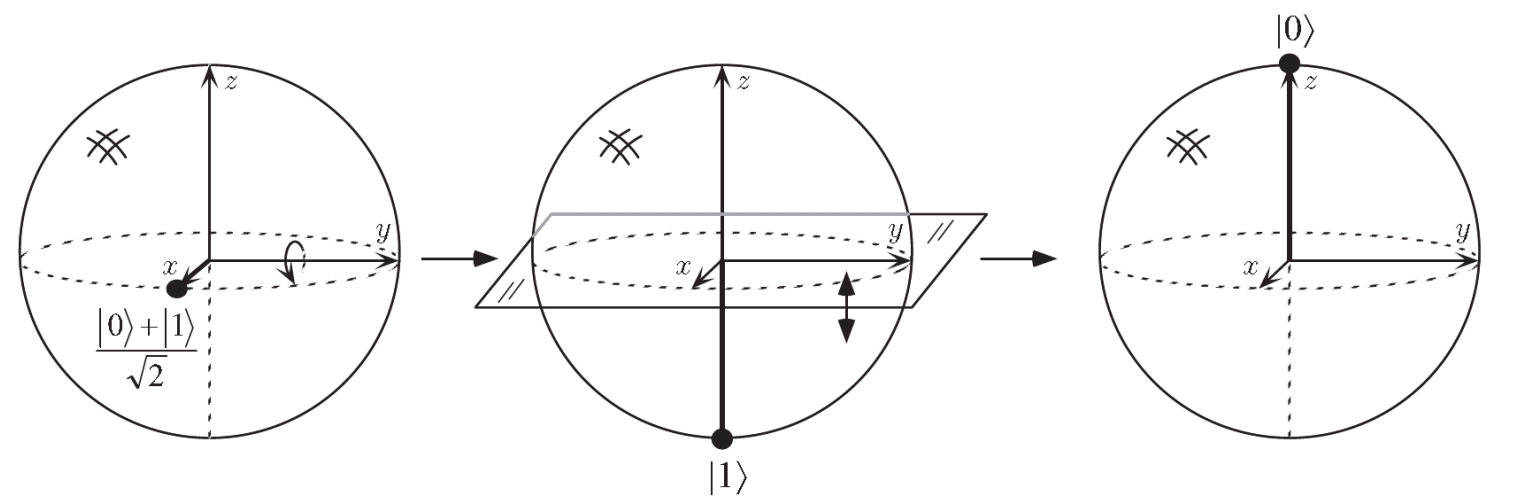
\includegraphics[width=12cm]{Images/Capitolo2/hadamard_sfera_bloch.png}
    \caption{Azione della porta Hadamard sullo stato $(|0\rangle + |1\rangle)/\sqrt{2}$.}
    \label{fig:hadamard_sfera_bloch}
\end{figure}

Prima di introdurre le porte rotazionali è necessario definire la matrice unitaria $u3$, la quale dipende da tre parametri: $\theta, \phi$ e $\lambda$.
\begin{equation}
    \label{eq:u3}
    u3(\theta,\phi,\lambda) =
    \begin{bmatrix}
       \cos{(\theta/2)} & e^{i\lambda}\sin{(\theta/2)}\\
        e^{i\phi}\sin{(\theta/2)} & e^{i\lambda+i\phi}\cos{(\theta/2)}
    \end{bmatrix}.
\end{equation}

Quest'ultima rappresenta una rotazione generica su di un qubit singolo e ci permette inoltre di riportare un qubit nel suo stato precedente.
Come vedremo, valorizzando correttamente questi tre parametri possiamo ottenere le porte rotazionali su tutti e tre gli assi.

Sapendo che qualsiasi matrice unitaria $2\times2$ si può decomporre come
\begin{equation}
    U=e^{i\alpha}
    \begin{bmatrix}
        e^{-i\beta/2} & 0\\
        0 & e^{i\beta/2}
    \end{bmatrix}
    \begin{bmatrix}
        \cos{\frac{\gamma}{2}} & -\sin{\frac{\gamma}{2}}\\
        \sin{\frac{\gamma}{2}} & \cos{\frac{\gamma}{2}}
    \end{bmatrix}
\end{equation}
è possibile costruire una qualsiasi porta a qubit singolo con un numero finito di porte quantistiche in quanto:
\begin{itemize}
    \renewcommand\labelitemi{--}
    \item il primo termine è un fattore di fase globale;
    \item la prima matrice rappresenta una rotazione attorno all'asse $\hat{z}$;
    \item la seconda matrice rappresenta una rotazione attorno all'asse $\hat{y}$.
\end{itemize}

Riuscendo quindi ad implementare le rotazioni attorno a questi assi, sarà possibile realizzare qualsiasi porta a qubit singolo, quindi ogni operazione di rotazione su ogni specifico asse può essere rappresentata con una matrice come raffigurato nelle Equazioni \ref{eq:rx}, \ref{eq:ry}, \ref{eq:rz}.
\begin{equation}
    \label{eq:rx}
    R_x(\theta) =
    \begin{bmatrix}
       \cos{(\theta/2)} & -i\sin{(\theta/2)}\\
        -i\sin{(\theta/2)} & \cos{(\theta/2)}
    \end{bmatrix} =
    u3(\theta,-\pi/2,\pi/2)
\end{equation}
\begin{equation}
    \label{eq:ry}
    R_y(\theta) =
    \begin{bmatrix}
       \cos{(\theta/2)} & -\sin{(\theta/2)}\\
        \sin{(\theta/2)} & \cos{(\theta/2)}
    \end{bmatrix} =
    u3(\theta,0,0)
\end{equation}
\begin{equation}
    \label{eq:rz}
    R_z(\phi) =
    \begin{bmatrix}
       e^{-i\phi/2} & 0\\
        0 & e^{i\phi/2}
    \end{bmatrix} =
    u1(\phi)
\end{equation}
Nella Figura \ref{fig:porte_logice_singolo_qubit} vengono inoltre riassunte e rappresentate graficamente le porte logiche $X$, $Z$ e $H$.
\begin{figure}[htp]
    \centering
    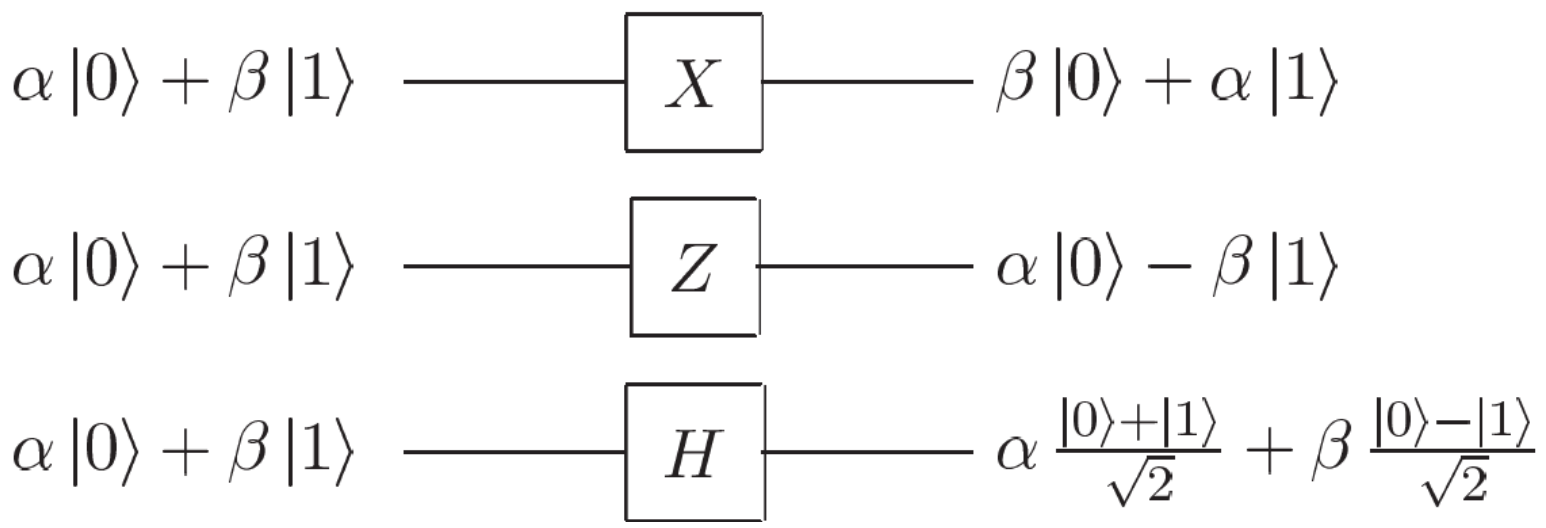
\includegraphics[width=8cm]{Images/Capitolo2/porte_logice_singolo_qubit.png}
    \caption{Esempio di porte a qubit singolo.}
    \label{fig:porte_logice_singolo_qubit}
\end{figure}
\newline
\subsection{Registri quantistici}
Con due bit classici possiamo formare quattro possibili stati: 00, 01, 10, 11.
In generale, con n bit è possibile costruire $2^n$ stati distinti.
Lo spazio degli stati generato da un sistema di n qubit ha dimensione $2^n$: ogni vettore normalizzato in questo spazio rappresenta un possibile stato computazionale, che chiameremo registro quantistico a n qubit.

Questa crescita esponenziale delle dimensioni dello spazio degli stati suggerisce la potenziale capacità di un computer quantistico di elaborare informazioni ad una velocità esponenzialmente superiore rispetto a quella di un computer classico.

Volendo definire formalmente un registro quantistico di n qubit possiamo considerarlo come un elemento dello spazio di Hilbert $2^n$-dimensionale, $\mathbb{C}^{{2}^n}$ con base computazionale formata da $2^n$ registri a n qubit
\begin{equation}
    |i\textsubscript{1}\rangle\otimes|i\textsubscript{2}\rangle\otimes \dotsm \otimes|i\textsubscript{n}\rangle
\end{equation}
con $i\textsubscript{j}\in\{0,1\}, 1 \leq j \leq n$.
Per convenienza il vettore sopra citato verrà scritto come $|i\textsubscript{1}\rangle|i\textsubscript{2}\rangle \dotsm |i\textsubscript{n}\rangle$ oppure $|i\textsubscript{1}i\textsubscript{2} \dotsm i\textsubscript{n}\rangle$.

\subsection{Porte a qubit multipli}
Al fine di implementare operazioni su due bit classici le porte logiche più importanti ed utilizzate sono AND, OR, XOR, NAND, NOR e NOT.

Le porte NOT e AND formano un insieme universale e quindi possono realizzare una qualsiasi funzione booleana, di conseguenza definiremo insieme universale anche la porta NAND.
Non essendo possibile risalire agli input a partire dai risultati, le porte classiche XOR e NAND non sono invertibili, pertanto non è possibile generalizzare le porte classiche a bit multipli con porte quantistiche a qubit multipli.

L'analogo quantistico di una porta universale è il NOT controllato o CNOT (controlled-NOT) che opera su due qubit: il primo è chiamato qubit di controllo mentre il secondo rappresenta il qubit target.
Se il controllo è zero allora il target non viene modificato, altrimenti se il controllo è 1 allora il target viene negato, cioè:
\begin{equation}
    |00\rangle\mapsto|00\rangle, |01\rangle\mapsto|01\rangle, |10\rangle\mapsto|11\rangle, |11\rangle\mapsto|10\rangle.
\end{equation}

Generalizzando una classica porta XOR possiamo vedere la CNOT con la seguente trasformazione:
\begin{equation}
    |A,B\rangle\mapsto|A, B\oplus A\rangle,
\end{equation}
dove $A$ è il qubit di controllo, $B$ è il target e $\oplus$ è la classica operazione XOR.
\begin{figure}[htp]
    \centering
    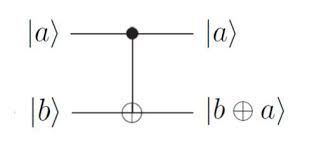
\includegraphics[width=6cm]{Images/Capitolo2/porta_cnot.png}
    \caption{Porta CNOT.}
    \label{fig:porta_cnot}
\end{figure}

Dopo aver visto la rappresentazione grafica del circuito in Figura \ref{fig:porta_cnot} andiamo a descrivere questa porta come matrice unitaria:
\begin{equation}
    CNOT= 
    \begin{bmatrix}
        1 & 0 & 0 & 0\\
        0 & 1 & 0 & 0\\
        0 & 0 & 0 & 1\\
        0 & 0 & 1 & 0
    \end{bmatrix}.
\end{equation}

A differenza delle porte classiche XOR e NAND, la CNOT è invertibile.
Quest'ultima, insieme a quelle a un qubit, rappresenta i prototipi di tutte le porte logiche quantistiche.

\section{Un esempio di circuito}
Ora che abbiamo introdotto tutte le principali porte logiche quantistiche, andiamo ad analizzare un circuito molto utile formato da una porta Hadamard ed una porta CNOT, come mostrato in Figura \ref{fig:circuito_bell}.
\begin{figure}[htp]
    \centering
    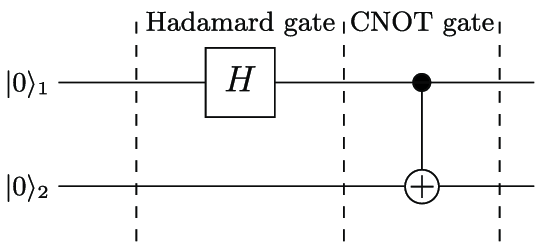
\includegraphics[width=8cm]{Images/Capitolo2/circuito_bell.png}
    \caption{Circuito per creare stati di Bell.}
    \label{fig:circuito_bell}
\end{figure}

Questo circuito trasforma i quattro stati fondamentali del sistema a due qubit in degli stati di Bell \cite{cambridge2010book}, o coppie EPR:
\begin{equation}
    |\beta_{00}\rangle =\dfrac{|00\rangle + |11\rangle}{\sqrt(2)}
\end{equation}
\begin{equation}
    |\beta_{01}\rangle =\dfrac{|01\rangle + |10\rangle}{\sqrt(2)}
\end{equation}
\begin{equation}
    |\beta_{10}\rangle =\dfrac{|00\rangle - |11\rangle}{\sqrt(2)}
\end{equation}\begin{equation}
    |\beta_{1}\rangle =\dfrac{|01\rangle - |10\rangle}{\sqrt(2)}
\end{equation}

La proprietà interessante di questo tipo di stati è che i qubit sono correlati; infatti la misura del secondo qubit restituirà sempre un risultato uguale a quella del primo. Bell dimostrò che questa correlazione viene mantenuta se si effettuano alcune operazioni sulla coppia EPR, prima di svolgere la misurazione dei qubit.

Dato quindi un input specifico, possiamo vedere nella Tabella \ref{table:verita_bell} quale sarà l'output risultante del circuito.
\begin{table}[ht]
\centering
\begin{tabular}{l|c}
    \hline\hline
    \textbf{In} &  \textbf{Out}\\
    \hline
    $|00\rangle$ & {$(|00\rangle + |11\rangle)/\sqrt{2}\equiv |\beta_{00}\rangle$}\\
    $|01\rangle$ & {$(|01\rangle + |10\rangle)/\sqrt{2}\equiv |\beta_{01}\rangle$}\\
    $|10\rangle$ & {$(|00\rangle - |11\rangle)/\sqrt{2}\equiv |\beta_{10}\rangle$}\\
    $|11\rangle$ & {$(|01\rangle - |10\rangle)/\sqrt{2}\equiv |\beta_{11}\rangle$}\\
    \hline\hline
\end{tabular}
\caption{Tabella di verità degli stati di Bell.}
\label{table:verita_bell}
\end{table}

\section{Algoritmi quantistici}
\subsection{Classi di complessità}
Nel mondo della computazione quantistica lo scopo principale è quello di trovare metodi o algoritmi migliori per individuare tutte le possibili soluzioni nella maniera più efficiente.

La teoria che si occupa di stabilire le risorse (tempo o spazio) necessarie per risolvere un determinato problema utilizzando uno specifico algoritmo, prende il nome di complessità computazionale: è quest'ultima a fare la differenza tra computer quantistici e computer classici.

L'obbiettivo è quello di individuare il metodo o l'algoritmo migliore, esplorando così l'intero spazio delle possibili soluzioni nella maniera più efficiente.
Questa problematica risulta essere non banale in quanto, se consideriamo n bit, lo spazio di ricerca contiene un numero di possibili soluzioni nell'ordine di $2^n$.

L'efficienza di un algoritmo è determinata da quanto il problema si presta o meno ad una strutturazione dello spazio delle possibili soluzioni e per misurarla bisogna tenere conto della crescita asintotica del tempo necessario ad ottenere il risultato (es. numero di passi dell'algoritmo) in funzione della dimensione dell'input ed è determinata da molteplici fattori.

Possiamo quindi definire un algoritmo efficiente per la teoria della complessità con uno per cui tale funzione è polinomiale in $n$ e, in corrispondenza, si dirà di ordine $O(n)$, $O(n^2)$, $O(n^3)$ ecc.
\begin{figure}[htp]
    \centering
    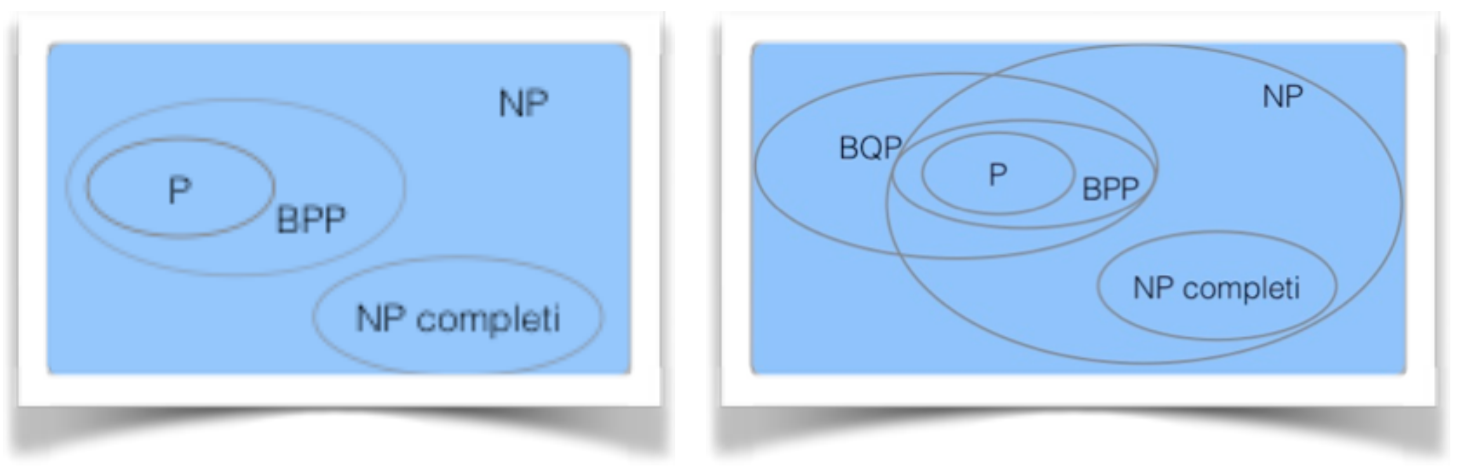
\includegraphics[width=12cm]{Images/Capitolo2/classi_complessita.png}
    \caption{Classi di complessità classiche e con BQP.}
    \label{fig:classi_complessita}
\end{figure}
\newline\newline

Andiamo ora ad approfondire ogni singola classe \cite{dipierro2013articolo}, prendendo come spunto i diagrammi in Figura \ref{fig:classi_complessita}:
\begin{itemize}
    \renewcommand\labelitemi{--}
    \item \textbf{\textit{P (Polynomial-time)}}, classe di tutti i problemi per cui esiste un algoritmo efficiente;
    \item \textbf{\textit{BPP (Bounded-error Probabilistic Polynomial-time)}}, classe dei problemi che possono essere risolti da algoritmi probabilistici in tempo polinomiale, con una probabilità di errore $<\dfrac{1}{3}$;
    \item \textbf{\textit{NP (Nondeterministic Polynomial-time)}}, classe dei problemi che possono essere risolti in tempo polinomiale, purché si utilizzi un algoritmo non deterministico;
    \begin{itemize}
        \item \textbf{\textit{NP completi}}, rappresentano i più difficili problemi non deterministici; un algoritmo in grado di risolvere "velocemente" un qualsiasi problema NP-C può essere utilizzato per risolvere "velocemente" ogni problema in NP;
    \end{itemize}
    \item \textbf{\textit{BQP (Bounded-error Quantum Polynomial-time)}}, classe dei problemi che richiedono da parte di un computer quantistico un tempo polinomiale, con una probabilità di errore $\leq\dfrac{1}{3}$.
\end{itemize}

La relazione presente tra le classi NP e BQP non è attualmente nota, come non è ancora nota l'esistenza di algoritmi efficienti per risolvere problemi NP-C.

\subsection{Teletrasporto quantistico}
Il primo argomento che andremo a trattare non sarà un algoritmo vero e proprio, piuttosto un interessante applicazione dell'elaborazione quantistica dell'informazione ed in particolare dell'entanglement.

Per il teorema di no-cloning quantistico \cite{wootters1982articolo}, copiare lo stato di un qubit è vietato, a meno che esso sia 0 o 1.
Tuttavia, nulla impedisce di teletrasportare \cite{cambridge2010book} il qubit a qualsiasi distanza, anche senza un canale di comunicazione quantistico.

Cerchiamo di fare un esempio considerando due persone fittizie, Alice e Bob.
Insieme, dopo essersi trovati, hanno creato uno stato di Bell.
In seguito si sono separati, prendendo ognuno uno dei due qubit entangled.
Una volta a grande distanza, l'obbiettivo di Alice è trasmettere a Bob, in uno stato sconosciuto, un nuovo qubit $|\psi \rangle=\alpha |0\rangle + \beta |1\rangle$.
Per farlo però, può usare soltanto canali di comunicazione classici (ovvero può spedire solo dei bit).
Grazie ai qubit entangled questo è possibile.

Il circuito è mostrato in Figura \ref{fig:teletrasporto_quantistico}.
Alice crea un sistema con il nuovo qubit e il suo qubit della coppia EPR.
Lo stato iniziale del sistema è
\begin{equation}
    |\psi_0\rangle = |\psi\rangle |\beta_{00}\rangle = \dfrac{1}{\sqrt{2}}[\alpha|0\rangle(|00\rangle + |11\rangle)+\beta|1\rangle(|00\rangle + |11\rangle)],
\end{equation}
dove i primi due qubit (sinistra) sono di Alice ed il terzo è di Bob.
Alice manda i suoi qubit in una porta CNOT, ottenendo
\begin{equation}
    |\psi_1\rangle = \dfrac{1}{\sqrt{2}}[\alpha|0\rangle (|00\rangle + |11\rangle)+\beta|1\rangle (|10\rangle + |01\rangle)].
\end{equation}

Alice manda poi il suo primo qubit in una porta Hadamard, ottenendo
\begin{equation}
    |\psi_2\rangle = \dfrac{1}{\sqrt{2}}[\alpha(|0\rangle + |1\rangle)(|00\rangle + |11\rangle) + \beta(|0\rangle - |1\rangle)(|10\rangle + |01\rangle)].
\end{equation}

Se raccogliamo i qubit di Alice, possiamo riscrivere l'equazione come
\begin{equation}
    \begin{split}
    |\psi_2\rangle =
    &\dfrac{1}{\sqrt{2}}[|00\rangle (\alpha|0\rangle + \beta|1\rangle)+|01\rangle(\alpha|1\rangle+\beta|0\rangle)+\\&+|10\rangle(\alpha|0\rangle-\beta|1\rangle)+|11\rangle(\alpha|1\rangle-\beta|0\rangle)].
    \end{split}
\end{equation}

A questo punto, Alice misura i suoi due qubit e manda il risultato a Bob. A seconda del risultato ottenuto, il sistema si troverà in uno di questi quattro stati:
\begin{gather}
 00 \longmapsto |\psi_3(00)\rangle = [\alpha|0\rangle + \beta|1\rangle]\\
 01 \longmapsto |\psi_3(01)\rangle = [\alpha|1\rangle + \beta|0\rangle]\\
 10 \longmapsto |\psi_3(10)\rangle = [\alpha|0\rangle - \beta|1\rangle]\\
 11 \longmapsto |\psi_3(11)\rangle = [\alpha|1\rangle - \beta|0\rangle]
\end{gather}

Per recuperare lo stato $\psi$ Bob deve applicare una porta quantistica che dipende dal risultato spedito da Alice.
Se il risultato è 00, Bob non deve applicare nulla.
Se il risultato è 01, Bob deve applicare una porta $X$.
Se il risultato è 10, Bob deve applicare una porta $Z$.
Se il risultato è 11, Bob deve applicare una porta $X$ e poi una porta $Z$.

Per riassumere, Bob deve applicare una porta $Z^{M_1}X^{M_2}$ (dove $M_1$ e $M_2$ sono i due bit inviati da Alice, e come nel prodotto matriciale viene applicato prima il termine sulla destra).
\begin{figure}[htp]
    \centering
    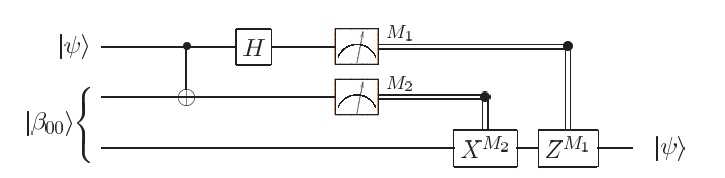
\includegraphics[width=13cm]{Images/Capitolo2/teletrasporto_quantistico.png}
    \caption[Circuito quantistico per il teletrasporto di un qubit.]{Circuito quantistico per il teletrasporto di un qubit. Le prime due linee rappresentano i qubit di Alice, mentre la terza il qubit di Bob.}
    \label{fig:teletrasporto_quantistico}
\end{figure}

Uno degli utilizzi più frequenti del teletrasporto quantistico, in ambito di computazione quantistica, riguarda la creazione di porte quantistiche che resistano al rumore.

\subsection{VQE}
\label{subsec:vqe}
L'algoritmo Variational Quantum Eigensolver (VQE) utilizzato nella fase sperimentale, che andremo ad implementare nell'Appendice \ref{codice:vqe}, ha l'obbiettivo di stimare le proprietà molecolari di un sistema quantistico utilizzando il principio variazionale.

Una proprietà molto spesso analizzata riguarda lo stato fondamentale di un atomo o di una molecola: l'utilizzo frequente di questo algoritmo ibrido trova applicazione nel campo della chimica computazionale quantistica.
Si definisce ibrido in quanto utilizza cicli alternati di calcolo classico e quantistico: nello specifico ci consente di trovare l'autovalore di una matrice H (solitamente di grandi dimensioni) attraverso una tecnica chiamata media Hamiltoniana.

Questa tecnica, in presenza di molti corpi, risulta difficile da studiare nei computer classici a causa della sua complessità e dimensionalità, mentre nei computer quantistici si hanno meno problemi di sovraccarico con conseguente crescita polinomiale.
Possiamo quindi schematizzare l'algoritmo VQE \cite{chimica_quantistica} nei seguenti passaggi:
\begin{enumerate}
    \item \textbf{\textit{Preparazione dello stato}}: uno stato quantistico parametrizzato $|\psi(\Vec{\theta})\rangle$ è preparato sul dispositivo quantistico. Questo grazie all'applicazione di un parametro unitario definito dalla scelta dell'\textit{ansatz}, il quale dovrebbe contenere una famiglia di stati non rappresentabili in maniera efficiente su di un computer classico;
    \item \textbf{\textit{Stima energetica}}: il valore atteso dall'energia $\langle H\rangle(\theta)$ è stimato utilizzando la procedura della media Hamiltoniana, la quale prevede la misurazione di prodotti tensoriali in termini di Pauli, corrispondenti alla rappresentazione del qubit;
    \item \textbf{\textit{Feedback classico}}: i parametri dello stato quantistico $\Vec{\theta}$ vengono aggiornati utilizzando una routine classica non lineare;
    \item I punti 2 e 3 vengono ripetuti finché i criteri di convergenza non sono soddisfatti.
\end{enumerate}

La struttura di base di VQE, rappresentata in Figura \ref{fig:struttura_vqe}, può essere definita modulare, in quanto lascia possibilità di futuri miglioramenti ed estensioni.
\begin{figure}[htp]
    \centering
    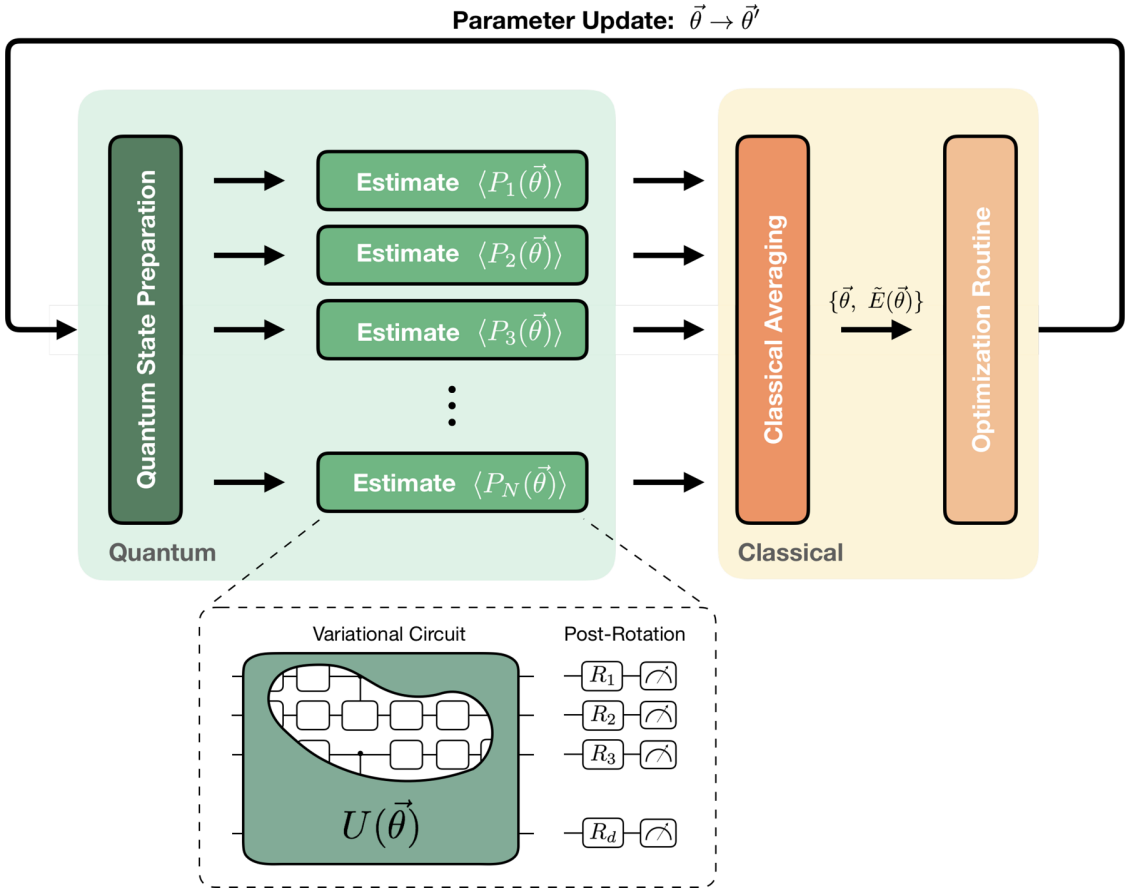
\includegraphics[width=\textwidth]{Images/Capitolo2/struttura_vqe.png}
    \caption{Illustrazione algoritmo VQE.}
    \label{fig:struttura_vqe}
\end{figure}
\newline\newline

\subsubsection{Equazione di Schrödinger}
Per introdurre questo argomento, dobbiamo prima definire il concetto di principio variazionale utilizzato nel paragrafo precedente; in generale questa tecnica ha lo scopo di risolvere un problema scientifico utilizzando il calcolo delle variazioni.

Nel nostro caso, parlando di meccanica quantistica \cite{sakai2018equazione}, quando calcoliamo il valore medio dell'operatore Hamiltoniano su una funzione d'onda arbitraria possiamo affermare che questo valore non sarà mai inferiore all'energia dello stato fondamentale.

Questo metodo risolve dunque l'equazione di Schrödinger (\ref{eq:equazione_schrodinger}), la quale rappresenta una delle più importanti conquiste della fisica ed in particolare della meccanica quantistica, consentendoci di trovare la \textit{funzione d'onda}, seno o coseno, che descrive il comportamento di una particella microscopica.
In termini più semplici, grazie ad essa riusciamo a calcolare le probabilità di trovare un elettrone nello spazio intorno al nucleo.

Definendo quindi l'Equazione \ref{eq:equazione_schrodinger} di Schrödinger e l'energia classica espressa come Hamiltoniana nell'Equazione \ref{eq:energia_hamiltoniana}, possiamo riscrivere la prima in maniera compatta:
\begin{equation}
    \label{eq:equazione_schrodinger}
    H(t)|\psi(t)\rangle=i\hbar\dfrac{\partial}{\partial t}|\psi(t)\rangle,
\end{equation}
\begin{equation}
    \label{eq:energia_hamiltoniana}
    H=\dfrac{p^{2}}{2m}+V(x),
\end{equation}
\begin{equation}
    \label{eq:sistema_qualsiasi_schrodinger}
    -\dfrac{\hbar^{2}}{2m}\dfrac{d^{2}\psi (x)}{dx^{2}}+V\psi (x)=E\psi (x),
\end{equation}
\begin{equation}
    \hat{H}\psi = E\psi,
\end{equation}
dove $\hat{H}$ rappresenta l'operatore Hamiltoniano.
\chapter{Fase sperimentale}
\fancyhead[RO, LE]{\bfseries Fase sperimentale}
Dopo aver introdotto le nozioni teoriche necessarie, possiamo finalmente passare alla parte sperimentale di questa tesi. Verrà descritto l'ambiente di sviluppo fino ad arrivare all'analisi dei risultati ottenuti, con i relativi grafici.

\section{Qiskit e la IBM Quantum Experience}
La piattaforma che ho utilizzato durante i vari esperimenti prende il nome di Qiskit (Quantum Information Science Kit): un framework open-source per la computazione quantistica fondato da IBM Research.

Ciò che ha spinto l'azienda a sviluppare uno strumento di questo tipo, insieme ed altre istituzioni accademiche, riguarda l'accesso al loro servizio di Cloud Quantum Computing denominato IBM Q Experience.
L'obbiettivo è quello di mettere a disposizione macchine quantistiche a favore di tutta la comunità scientifica, toccando con particolare interesse alcuni settori di ricerca; queste macchine possono essere liberamente utilizzate sia per scopi di ricerca che a puro scopo didattico.

La versione principale e più utilizzata di Qiskit è basata sul linguaggio Python, attraverso il quale si possono creare programmi basati sulla rappresentazione Open-QASM \cite{larose2019articolo, assembly2017articolo} dei circuiti quantistici.

Richiamando all'occorrenza delle apposite API \cite{qiskit2018articolo} è possibile comunicare con i dispositivi IBM, così da far eseguire porzioni di codice a macchine reali o simulatori, i quali permettono di ottenere i risultati ideali.
Il servizio IBM Q Experience può essere utilizzato all'interno del sito, senza bisogno di installare nessun pacchetto.
Quest'ultimo mette a disposizione diversi esempi per avvicinarsi a questi temi, che variano dal più semplice al più complesso; è inoltre presente una piattaforma grafica chiamata Circuit Composer in cui è possibile realizzare circuiti trascinando elementi.

Nella Tabella \ref{table:dispositivi_quantistici} è possibile vedere alcuni dei backend disponibili gratuitamente, con relativo numero di qubit.
\begin{table}[h]
\centering
\begin{tabular}{l|c|c}
    \hline\hline
    \textbf{Nome macchina} &  \textbf{Num.qubits} & \textbf{Simulatore}\\
    \hline
    \textit{ibmq\_santiago} & 5 &  \\
    \textit{ibmq\_athens} & 5 &  \\
    \textit{ibmq\_vigo} & 5 &  \\
    \textit{ibmq\_valencia} & 5 &  \\
    \textit{ibmq\_16\_melbourne} & 15 &  \\
    \textit{ibmq\_ourense} & 5 &  \\
    \textit{ibmq\_qasm\_simulator} & {Up to 32} & $\times$\\
    \hline\hline
\end{tabular}
\caption{Alcuni dei dispositivi IBM disponibili.}
\label{table:dispositivi_quantistici}
\end{table}
\newline\newline

Una volta creati e lanciati gli esperimenti, l'utente dovrà attendere un lasso di tempo che potrà essere influenzato o meno dalla coda presente nel dispositivo.
La complessità dell'esperimento avviato richiederà a sua volta una mole di tempo variabile per essere portato a termine.

\subsection{Elementi di Qiskit}
Qiskit\footnote{Qiskit: An Open-source Framework for Quantum Computing, 2019, \url{https://doi.org/10.5281/zenodo.2562111}}  è una libreria di Python dedicata al calcolo quantistico, suddivisa in quattro grandi sotto-librerie, ognuna con un ambito ben preciso e specifico, come si può evincere dalla Figura \ref{fig:elementi_qiskit}.
\begin{itemize}
    \renewcommand\labelitemi{--}
    \item \textbf{\textit{Terra}}, fornisce una base per la creazione di programmi quantistici a livello di circuiti ed impulsi, definendo inoltre le interfacce utilizzabili dall'utente finale il quale potrà comunicare con i dispositivi remoti;
    \item \textbf{\textit{Aer}}, ci aiuta a comprendere i limiti dei processori classici dimostrando fino a che punto possono imitare il calcolo quantistico, include al suo interno vari simulatori scritti in C++ ottimizzati per l'esecuzione di circuiti compilati in Terra, consentendo inoltre di verificare se i computer attuali e futuri funzionino correttamente;
    \item \textbf{\textit{Ignis}}, è pensato per coloro che vogliono progettare codici di correzione degli errori quantistici, permettendo una migliore caratterizzazione degli stessi ed un perfezionamento delle porte durante l'elaborazione in presenza di rumore;
    \item \textbf{\textit{Aqua}}, racchiude al suo interno una serie di algoritmi quantistici che trovano applicazioni nel mondo reale, in particolare i domini d'interesse risultano essere la chimica, l'ottimizzazione, la finanza e l'intelligenza artificiale.
\end{itemize}
\begin{figure}[htp]
    \centering
    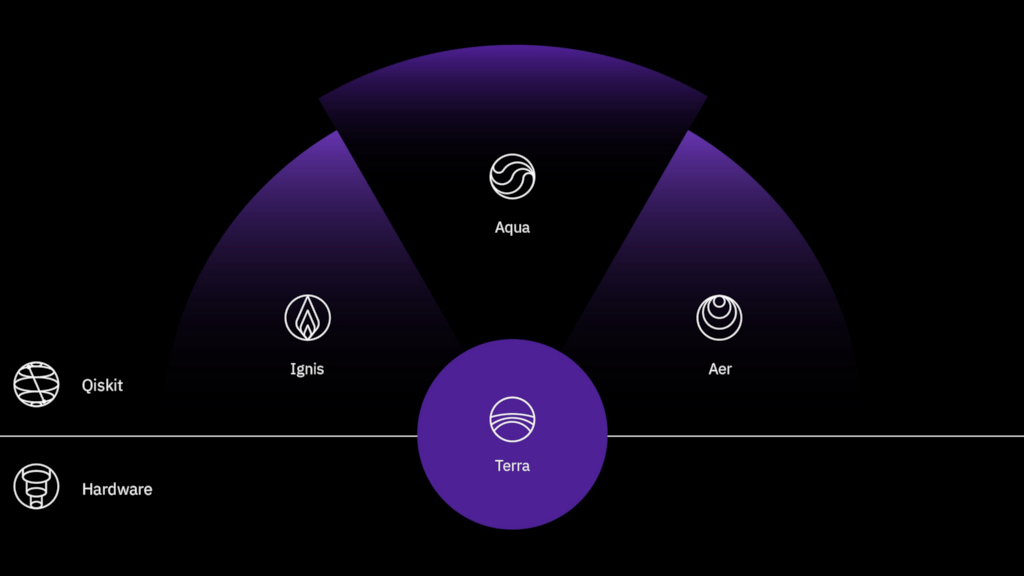
\includegraphics[width=13cm]{Images/Capitolo3/elementi_qiskit.png}
    \caption{Schema elementi di Qiskit.}
    \label{fig:elementi_qiskit}
\end{figure}

\section{Descrizione del sistema}
Come abbiamo visto nel Paragrafo \ref{subsec:vqe}, per implementare l'algoritmo VQE è necessario definire un circuito parametrico quantistico.
Quest'ultimo ci permette di effettuare la stima energetica della molecola presa in esame attraverso il susseguirsi di operazioni, specificate da porte logiche quantistiche.

Ora andremo ad analizzare in dettaglio i due circuiti utilizzati, sia dal punto di vista grafico che strutturale.
\subsection{TwoLocal}
Il circuito TwoLocal è parametrizzato in quanto costituito da strati di rotazione alternati e strati di entanglement.
Le rotazioni vengono specificate attraverso porte a qubit singolo ed applicate su tutti i qubit, lo strato di entanglement invece, utilizza porte a due qubit per intrecciare quest'ultimi secondo una delle seguenti strategie: \textit{full}, \textit{linear}, \textit{circular} e \textit{sca}.

Si può vedere una sua rappresentazione con full entanglement in Figura \ref{fig:circuito_twolocal}.
\begin{figure}[htp]
    \centering
    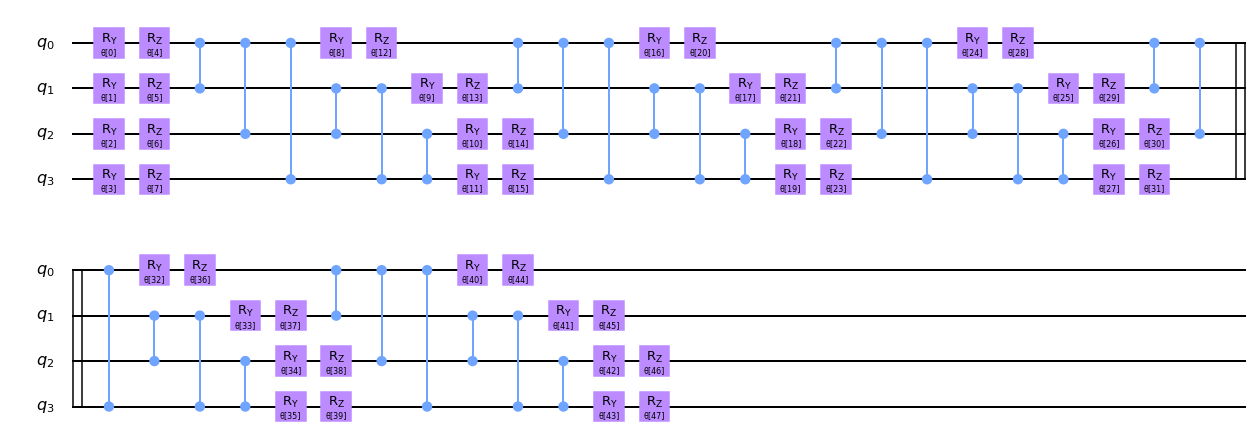
\includegraphics[width=13cm]{Images/Capitolo3/circuito_twolocal.png}
    \caption[Schema circuito TwoLocal.]{Schema circuito TwoLocal con full entanglement e porte logiche RY, RZ e CZ.}
    \label{fig:circuito_twolocal}
\end{figure}

\subsection{EfficientSU2}
Il circuito EfficientSU2 è costituito da strati di operazioni a qubit singolo, attraversato da intrecci SU(2) e $CX$ entanglement.
Questo è un modello euristico che può essere utilizzato per preparare funzioni d'onda di prova per algoritmi quantistici variazionali o circuiti di classificazione per l'apprendimento automatico.

SU(2) sta per gruppo unitario speciale di grado 2, i suoi elementi sono matrici unitarie $2\times2$ con determinante uguale a 1, come le porte di rotazione di Pauli.

Si può vedere una sua doppia rappresentazione, la prima in Figura \ref{fig:circuito_efficientsu2_linear} con linear entanglement mentre la seconda in Figura \ref{fig:circuito_efficientsu2_full} con full entanglement.
\begin{figure}[htp]
    \centering
    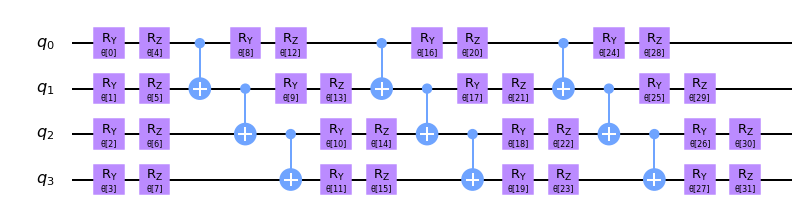
\includegraphics[width=12cm]{Images/Capitolo3/circuito_efficientsu2_linear.png}
    \caption{Schema circuito EfficientSU2 con linear entanglement.}
    \label{fig:circuito_efficientsu2_linear}
\end{figure}
\begin{figure}[htp]
    \centering
    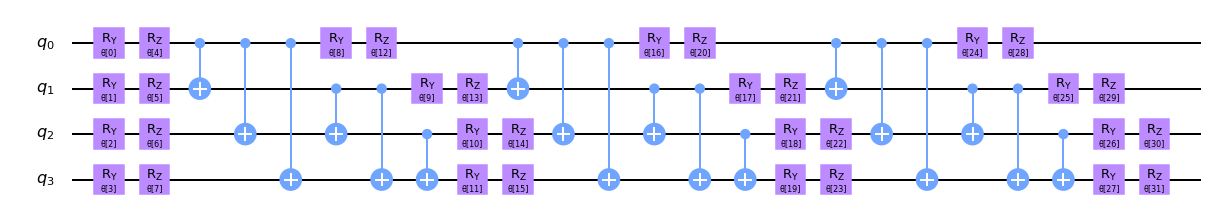
\includegraphics[width=13cm]{Images/Capitolo3/circuito_efficientsu2_full.png}
    \caption{Schema circuito EfficientSU2 con full entanglement.}
    \label{fig:circuito_efficientsu2_full}
\end{figure}
\newline

\section{Passaggi preliminari}
\subsection{Preparazione dell'ambiente di sviluppo}
Per utilizzare Qiskit è necessario avere installato nel proprio terminale il linguaggio di programmazione Python, versione 3.5 o successive; si ha inoltre piena compatibilità con i più diffusi sistemi operativi (Windows, macOS e Linux).
Il modo migliore per utilizzare questo framework è quello di installare un ambiente virtuale all'interno della propria macchina locale o su cloud, così da separare Qiskit dalle altre applicazione ed avere un'esperienza d'uso migliore.

I passi da me svolti per preparare l'ambiente di sviluppo nel sistema operativo Ubuntu sono stati quindi i seguenti:
\begin{enumerate}
    \item installare Anaconda e creare un ambiente minimale con solo Python al suo interno;
    \begin{itemize}
        \item[$\$$] \mintinline{bash}{conda create -n name_of_my_env python=3}
    \end{itemize}
    \item attivare l'ambiente appena creato;
    \begin{itemize}
        \item[$\$$] \mintinline{bash}{conda activate name_of_my_env}
    \end{itemize}
    \item installare Qiskit tramite il gestore dei pacchetti di Python (pip);
    \begin{itemize}
        \item[$\$$] \mintinline{bash}{pip install qiskit}
    \end{itemize}
    \item utilizzare Jupyter Notebook per interagire con Qiskit ed iniziare a svolgere i primi esperimenti.
\end{enumerate}

\subsection{Autenticazione all'IBM Quantum Systems}
Abbiamo visto come IBM metta a disposizione il suo servizio di Cloud Quantum Computing denominato IBM Q Experience, per utilizzarlo e configurarlo correttamente con Qiskit ho dovuto seguire i passi qui in elenco:
\begin{enumerate}
    \item creare gratuitamente un account IBM Q Experience;
    \item navigare nella sezione \say{My Account} e copiare il token disponibile nella casella di testo, così da poter accedere all'API;
    \item eseguire questi comandi in Jupyter per archiviare localmente il token API, sostituendo MY\_API\_TOKEN con il valore copiato;
    \begin{itemize}
        \item[] \mintinline{python}{from qiskit import IBMQ} \\
                \mintinline{python}{IBMQ.save_account('MY_API_TOKEN')}
    \end{itemize}
\end{enumerate}

\section{Analisi del problema}
Come già accennato in precedenza, si cercherà di utilizzare l'algoritmo ibrido VQE, all'interno un sistema quantistico simulato ideale, denominato da Qiskit \textit{statevector}.

Al fine di poter confrontare i dati ed i grafici ottenuti da queste simulazioni si è deciso di applicare allo stesso problema un algoritmo classico, chiamato NumpyMinumEigenSolver, il quale utilizza a sua volta l'operatore Hamiltoniano per ricavare i valori dell'energia di legame.

Il problema, analizzato principalmente a livello teorico da chi studia chimica computazionale, ci ha permesso di misurare l'energia propagata da una molecola in funzione dell'interdistanza atomica tra gli atomi costituenti.

La molecola sulla quale sono stati fatti il maggior numero di esperimenti è l'Idrogeno ($H_2$) essendo la più semplice a livello di struttura, mentre un numero inferiore di esperimenti è stato fatto anche per l'Idruro di Litio ($LiH$), il quale ha richiesto tempi di esecuzione molto più lunghi.

Le prime simulazioni sono state fatte utilizzando il backend denominato BasicAer, scritto in Python ed attualmente definito obsoleto, per questo motivo si è poi passati all'utilizzo del backend Aer, scritto in C++ e perciò più prestante.
Il metodo di simulazione specificato per entrambi i backend è stato \textit{statevector\_simulator}; a seconda della configurazione scelta ho potuto aggiungere l'opzione \textit{statevector\_gpu} al fine di utilizzare la potenza di calcolo della scheda video.

Una volta decisi questi parametri è stato necessario scegliere un ottimizzatore locale, ossia una funzione che tenta di trovare un valore ottimale all'interno di un range; quello su cui è stato fatto il maggior numero di prove è L\_BFGS\_B ma ne sono stati testati anche altri.

\subsection{Risultati ottenuti}
Le macchine che sono state utilizzate per effettuare i test sono 3; ne verranno elencate di seguito le caratteristiche sia hardware che software e ad ogni configurazione verrà associato un nome identificativo.
\small
\begin{itemize}
    \item \textbf{Notebook\_CPU} - Ubuntu 19.10 - i7-8750H - 16GB
    \item \textbf{Notebook\_GPU} - Ubuntu 19.10 - i7-8750H - GTX 1050 Ti - 16GB
    \item \textbf{Colab\_CPU} - Linux - Backend Google Compute Engine - 12.72GB
    \item \textbf{Colab\_GPU} - Linux - Backend (GPU) Google Compute Engine - 12.72GB
    \item \textbf{Tower\_GPU} - Windows 10 v2004 build 20236.1005 - Ubuntu 20.04 on WSL2 - i5-6600K - GTX 1070 - 16GB
\end{itemize}
\normalsize

Ogni tabella nella prima riga evidenzia il nome identificativo del dispositivo ed il backend utilizzato; se il dispositivo avrà come sigla finale \say{CPU} l'opzione specificata sarà \textit{statevector}, altrimenti nel caso di \say{GPU}, verrà utilizzata l'accelerazione hardware attraverso la direttiva \textit{statevector\_gpu}.

Se non diversamente specificato si farà riferimento a test svolti sulla molecola d'Idrogeno $H_2$ ed i tempi di esecuzione verranno indicati secondo lo standard ISO 8601 (hh:mm:ss,ms).

Ogni grafico sarà formato da due curve che rappresentano rispettivamente i differenti metodi utilizzati per calcolare l'energia di legame.
In azzurro si ha la curva definita attraverso il metodo d'approssimazione d'onda di Hartree-Fock, il quale minimizza l'energia totale presente all'interno della molecola; in arancione si può vedere invece la curva generata da uno dei due algoritmi da noi utilizzati: NumPyMinimumEigensolver o VQE.
Nei punti in cui il valore dell'ordinata raggiunge il suo estremo inferiore ci troveremo nello stato fondamentale della molecola, ovvero il punto in cui l'energia contenuta in essa è minima, da qui in poi le due curve risulteranno simili con variazioni assunte nelle coordinate $y$.

\subsubsection{L\_BFGS\_B}
L'obiettivo di Broyden-Fletcher-Goldfarb-Shanno Bound a memoria limitata è di minimizzare il valore differenziabile di una funzione scalare $f$.

Questo ottimizzatore non richiede l'hessiana di $f$ (la matrice delle derivate seconde di $f$) quando si tenta di calcolare il valore minimo della funzione, bensì effettua una stima iniziale del valore ottimale e procede iterativamente per perfezionare tale stima con una sequenza di stime migliori, risolvendo così problemi di ottimizzazione non vincolata e non lineare.

Nel nostro caso andremo ad eseguire un massimo di 2500 valutazioni di funzioni.

%-------------------------------------------------------------------------------------------------------
% NumPyMinimumEigensolver
\begin{figure}[htp]
    \centering
    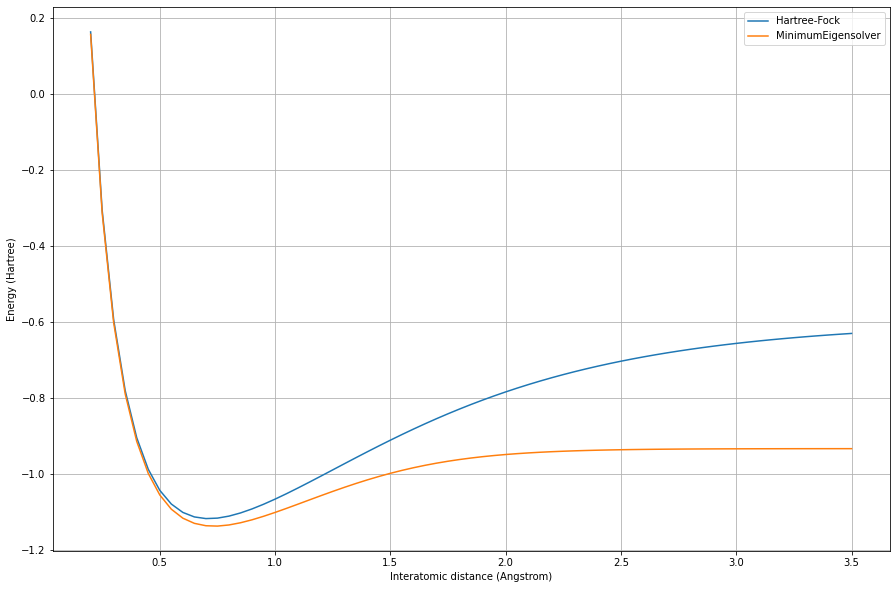
\includegraphics[width=8cm]{Images/Capitolo3/Plots/H2_numpy_minimum_eigensolver_plot.png}
    \caption[Grafico atteso \newline H2 NumPyMinimumEigensolver.]{}
    \label{fig:numpy_minimum_eigensolver}
\end{figure}
\noindent
\newline
Il grafico mostrato in Figura \ref{fig:numpy_minimum_eigensolver} rappresenta il risultato atteso, ottenuto attraverso il metodo del calcolo degli autovalori dell'Hamiltoniano utilizzando l'algoritmo classico NumPyMinimumEigensolver.
\newline
%-------------------------------------------------------------------------------------------------------
% PRIMO TEST - Notebook_CPU - BasicAer
\begin{minipage}[b]{0.39\textwidth}
    \scalebox{0.8}{%
    \begin{tabular}[b]{l|c}
        \hline\hline
        \multicolumn{2}{c}{\textbf{\textit{Notebook\_CPU - BasicAer}}}\\
        \hline
        \multirow{3}{*}{\textit{TwoLocal}} & 33:49,7277235984804\\
        \cline{2-2} & 32:36,4913177490235\\
        \cline{2-2} & 33:08,7257981300354\\
        \hline\hline
    \end{tabular}}
    \captionsetup{type=table}
    \caption[Risultati prima simulazione.]{Nella colonna di destra sono riportati i tempi di esecuzione.}
    \label{table:notebookcpu_basicaer}
\end{minipage}
\hfill
\begin{minipage}[b]{0.59\textwidth}
    \centering
    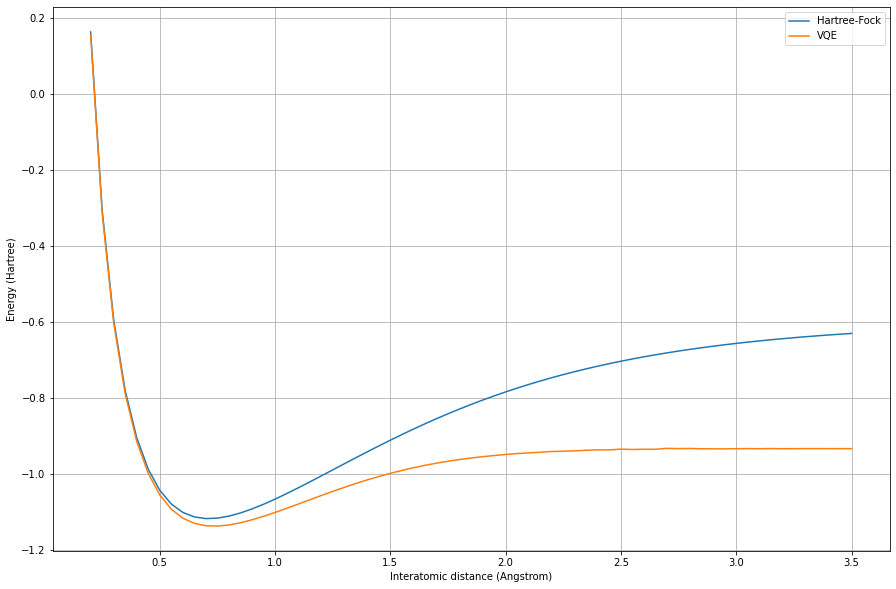
\includegraphics[width=1.0\textwidth]{Images/Capitolo3/Plots/H2_twolocal_ry_rz_cz_basic_cpu_plot.png}
    \captionof{figure}[Grafico 1 \newline TwoLocal - L\_BFGS\_B - Notebook\_CPU - BasicAer.]{}
    \label{fig:notebookcpu_basicaer}
\end{minipage}
\noindent
La prima simulazione è stata eseguita su Notebook\_CPU, con circuito TwoLocal e backend BasicAer.
Nella Tabella \ref{table:notebookcpu_basicaer} possiamo notare come i tempi di esecuzione hanno superato di poco la mezz'ora ed il grafico risultante, mostrato in Figura \ref{fig:notebookcpu_basicaer}, è praticamente identico a quello desiderato.
%-------------------------------------------------------------------------------------------------------
% SECONDO TEST - Notebook_CPU - Aer
\begin{minipage}[b]{0.39\textwidth}
    \scalebox{0.7}{%
    \begin{tabular}[b]{l|c}
        \hline\hline
        \multicolumn{2}{c}{\textbf{\textit{Notebook\_CPU - Aer}}}\\
        \hline
        \multirow{3}{*}{\textit{TwoLocal}} & 19:28,805236419042\\
        \cline{2-2} & 19:02,921885251999\\
        \cline{2-2} & 19:10,1750914255778\\
        \hline
        \multirow{3}{6em}{\textit{EfficientSU2 (linear)}} & 12:38,4950276215871\\
        \cline{2-2} & 12:38,0117837587992\\
        \cline{2-2} & 13:31,9865949948628\\
        \hline
        \multirow{3}{6em}{\textit{EfficientSU2 (full)}} & 13:04,8190720876057\\
        \cline{2-2} & 12:55,1782127221426\\
        \cline{2-2} & 13:19,6319488684336\\
        \hline\hline
    \end{tabular}}
    \captionsetup{type=table}
    \caption[Risultati seconda simulazione.]{Nella colonna di destra sono riportati i tempi di esecuzione.}
    \label{table:notebookcpu_aer}
\end{minipage}
\hfill
\begin{minipage}[b]{0.57\textwidth}
    \centering
    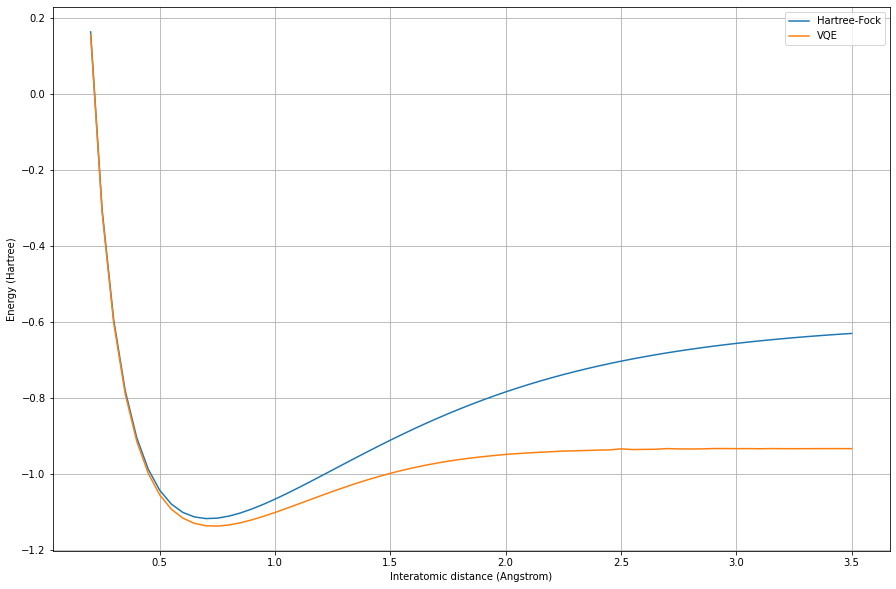
\includegraphics[width=1.0\textwidth]{Images/Capitolo3/Plots/H2_twolocal_ry_rz_cz_aer_cpu_plot.png}
    \captionof{figure}[Grafico 2 \newline TwoLocal - L\_BFGS\_B - Notebook\_CPU - Aer.]{}
    \label{fig:notebookcpu_twolocal_aer}
\end{minipage}
\begin{figure}[h]
    \begin{subfigure}[h]{0.49\linewidth}
        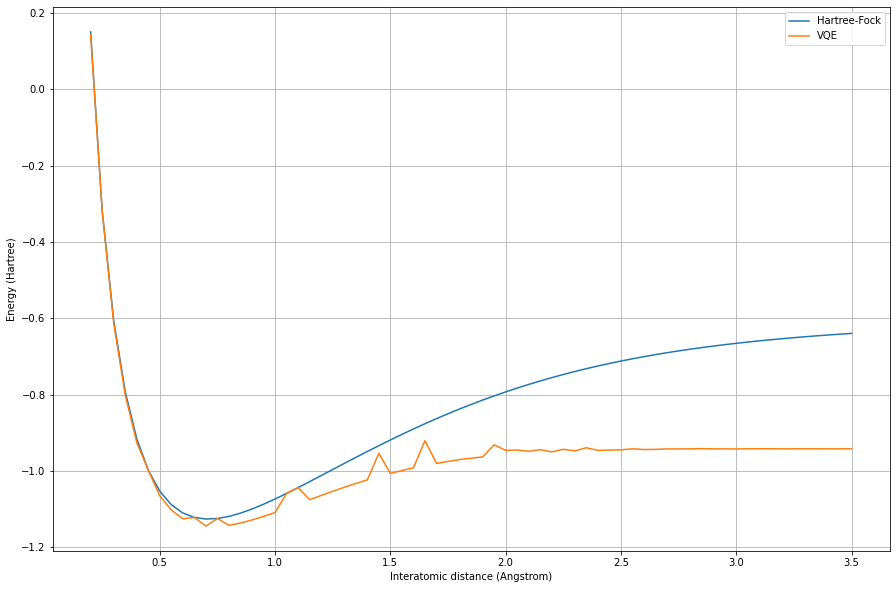
\includegraphics[width=0.80\linewidth]{Images/Capitolo3/Plots/H2_efficientsu2_linear_aer_cpu_plot.png}
        \caption{Linear}
    \end{subfigure}
    \hfill
    \begin{subfigure}[h]{0.49\linewidth}
        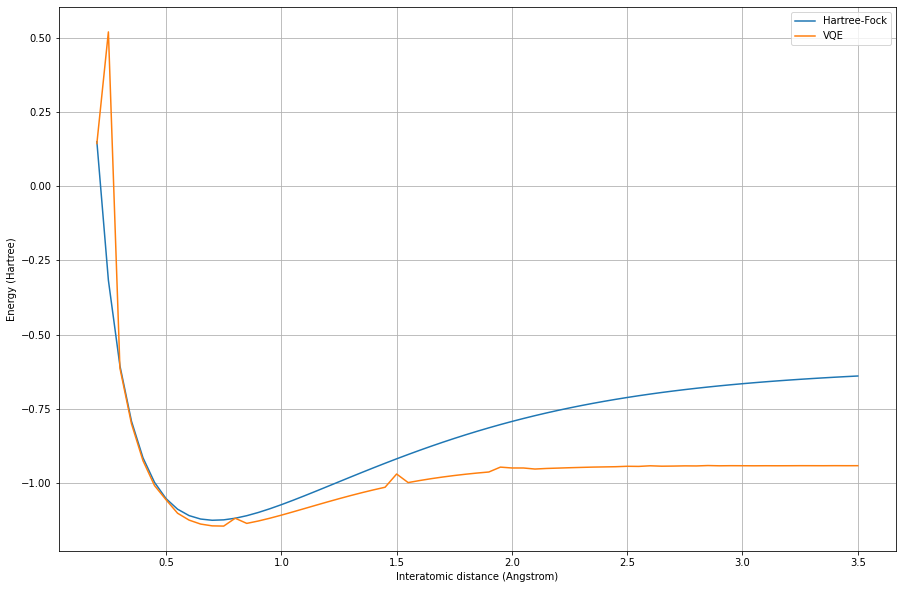
\includegraphics[width=0.80\linewidth]{Images/Capitolo3/Plots/H2_efficientsu2_full_aer_cpu_plot.png}
        \caption{Full}
    \end{subfigure}%
    \caption[Grafico 3 \newline EfficientSU2 - L\_BFGS\_B - Notebook\_CPU - Aer.]{}
    \label{fig:notebookcpu_efficientsu2_aer}
\end{figure}
\newline
La seconda simulazione è stata eseguita su Notebook\_CPU sia con il circuito TwoLocal che EfficientSU2 (linear/full entanglement).
Guardando la Tabella \ref{table:notebookcpu_aer} possiamo subito notare come il backend Aer abbia inciso nei tempi di esecuzione rispetto alla simulazione precedente ed anche in questo caso il grafico mostrato in Figura \ref{fig:notebookcpu_twolocal_aer} non presenta differenze sostanziali da quello desiderato.
Diverso è invece per il secondo circuito (\ref{fig:notebookcpu_efficientsu2_aer}) che pur avendo tempi di esecuzione minori, presenta molteplici picchi.
%-------------------------------------------------------------------------------------------------------
% TERZO TEST - Colab_CPU - Aer
\begin{minipage}[b]{0.39\textwidth}
    \scalebox{0.7}{%
    \begin{tabular}[b]{l|c}
        \hline\hline
        \multicolumn{2}{c}{\textbf{\textit{Colab\_CPU - Aer}}}\\
        \hline
        \multirow{3}{*}{\textit{TwoLocal}} & 21:16,5351521968842\\
        \cline{2-2} & 23:56,1901756127675\\
        \cline{2-2} & 23:26,9021610418955\\
        \hline\hline
    \end{tabular}}
    \captionsetup{type=table}
    \caption[Risultati terza simulazione.]{Nella colonna di destra sono riportati i tempi di esecuzione.}
    \label{table:colabcpu_aer}
\end{minipage}
\hfill
\begin{minipage}[b]{0.57\textwidth}
    \centering
    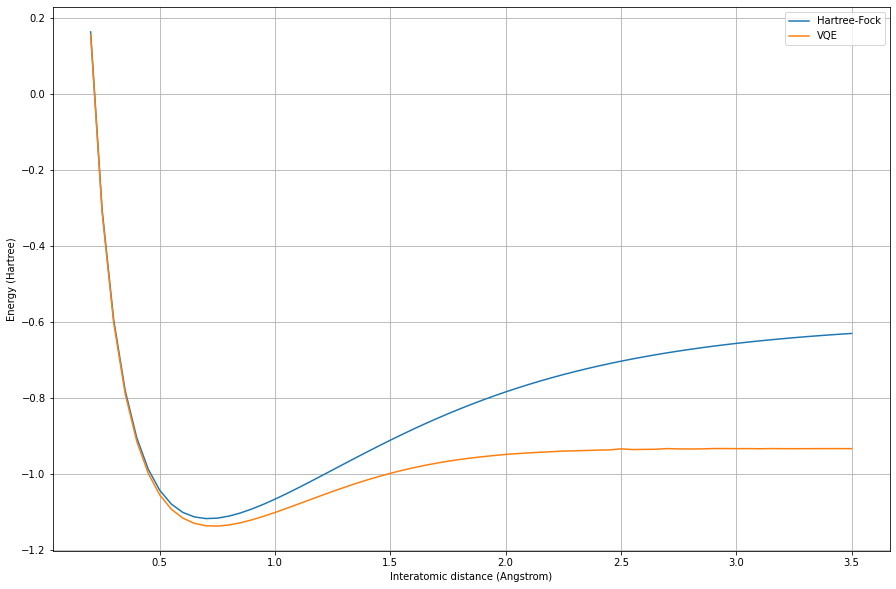
\includegraphics[width=1.0\textwidth]{Images/Capitolo3/Plots/H2_twolocal_ry_rz_cz_aer_cpu_plot.png}
    \captionof{figure}[Grafico 4 \newline TwoLocal - L\_BFGS\_B - Colab\_CPU - Aer.]{}
    \label{fig:colabcpu_twolocal_aer}
\end{minipage}
% Stesso plot di twolocal_ry_rz_cz_aer_cpu
\newline
La terza simulazione è stata eseguita su Colab\_CPU con il solo circuito TwoLocal e backend Aer.
I tempi ottenuti con la macchina messa a disposizione da Google, visibili nella Tabella \ref{table:colabcpu_aer}, sono risultati di poco peggiori rispetto ai test precedenti.
Il grafico, visibile in Figura \ref{fig:colabcpu_twolocal_aer}, rispecchia allo stesso modo il risultato atteso.
\newline\newline
%-------------------------------------------------------------------------------------------------------
% QUARTO TEST - Notebook_GPU - Aer
\begin{minipage}[b]{0.39\textwidth}
    \scalebox{0.7}{%
    \begin{tabular}[b]{l|c}
        \hline\hline
        \multicolumn{2}{c}{\textbf{\textit{Notebook\_GPU - Aer}}}\\
        \hline
        \multirow{3}{*}{\textit{TwoLocal}} & 20:28,53897968928\\
        \cline{2-2} & 20:41,6204098860423\\
        \cline{2-2} & 20:37,403276761373\\
        \hline
        \multirow{3}{6em}{\textit{EfficientSU2 (linear)}} & 13:14,5505837599437\\
        \cline{2-2} & 12:58,8811322053273\\
        \cline{2-2} & 12:27,9368682702382\\
        \hline
        \multirow{3}{6em}{\textit{EfficientSU2 (full)}} & 13:41,7947971820832\\
        \cline{2-2} & 13:39,1802767912546\\
        \cline{2-2} & 13:37,501518726349\\
        \hline\hline
    \end{tabular}}
    \captionsetup{type=table}
    \caption[Risultati quarta simulazione.]{Nella colonna di destra sono riportati i tempi di esecuzione.}
    \label{table:notebookgpu_aer}
\end{minipage}
\hfill
\begin{minipage}[b]{0.57\textwidth}
    \centering
    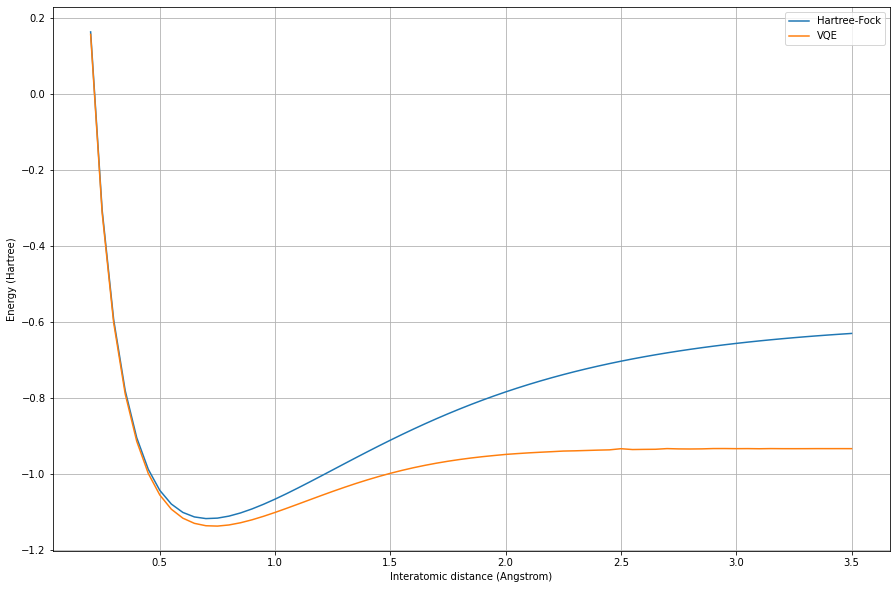
\includegraphics[width=1.0\textwidth]{Images/Capitolo3/Plots/H2_twolocal_ry_rz_cz_aer_gpu_plot.png}
    \captionof{figure}[Grafico 5 \newline TwoLocal - L\_BFGS\_B - Notebook\_GPU - Aer.]{}
    \label{fig:notebookgpu_twolocal_aer}
\end{minipage}
\begin{figure}[t]
    \begin{subfigure}[h]{0.49\linewidth}
        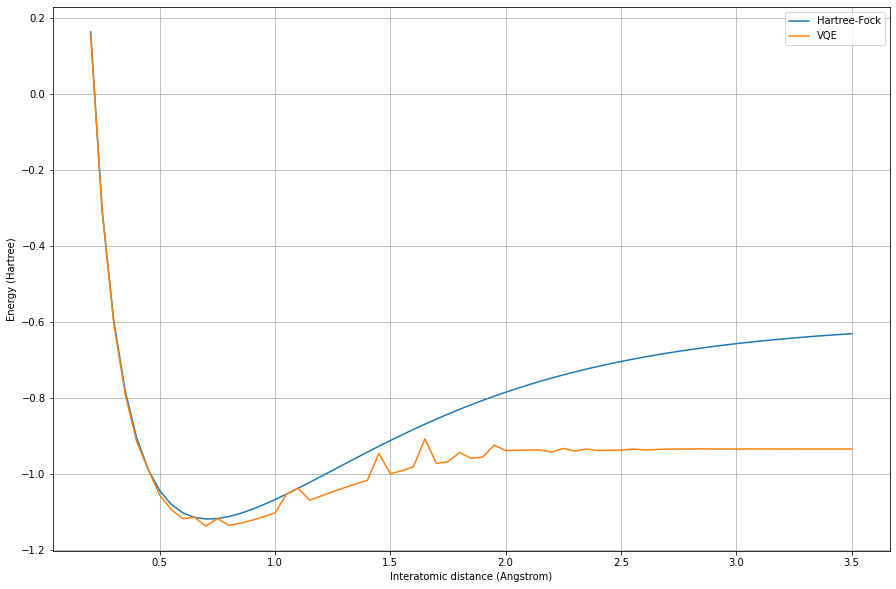
\includegraphics[width=\linewidth]{Images/Capitolo3/Plots/H2_efficientsu2_linear_aer_gpu_plot.png}
        \caption{Linear}
    \end{subfigure}
    \hfill
    \begin{subfigure}[h]{0.49\linewidth}
        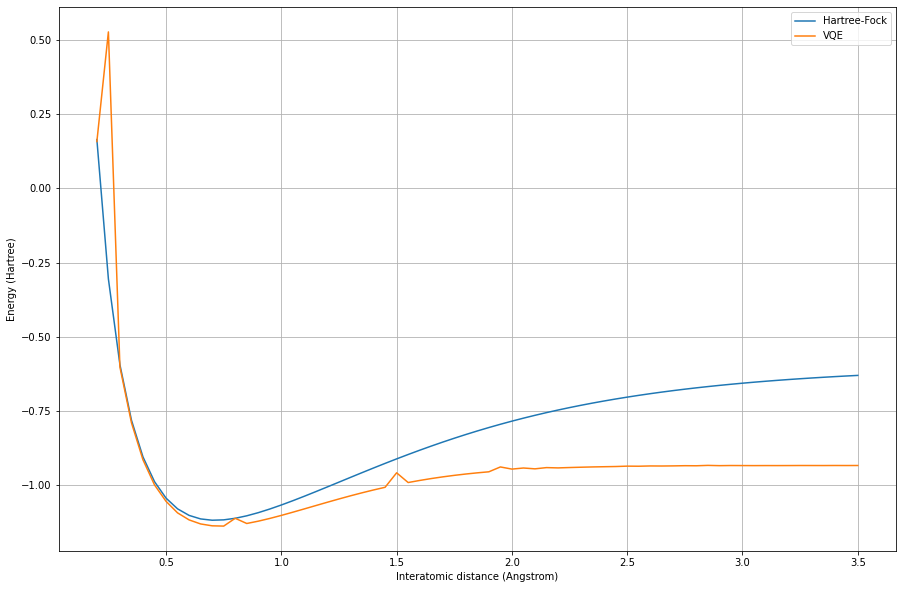
\includegraphics[width=\linewidth]{Images/Capitolo3/Plots/H2_efficientsu2_full_aer_gpu_plot.png}
        \caption{Full}
    \end{subfigure}%
    \caption[Grafico 6 \newline EfficientSU2 - L\_BFGS\_B - Notebook\_GPU - Aer.]{}
    \label{fig:notebookgpu_efficientsu2_aer}
\end{figure}
\newline\newline
Nella quarta simulazione abbiamo iniziato ad utilizzare la GPU, aspettandoci quindi dei tempi di esecuzione inferiori.
Purtroppo così non è stato, come si può notare dalla Tabella \ref{table:notebookgpu_aer}.
Il test è stato eseguito su Notebook\_GPU con entrambi i circuiti e backend Aer, i grafici mostrati nelle Figure \ref{fig:notebookgpu_twolocal_aer} e \ref{fig:notebookgpu_efficientsu2_aer} rimangono i medesimi visti in precedenza.
%-------------------------------------------------------------------------------------------------------

Per verificare che effettivamente questi risultati non dipendano dalla scarsa potenza della scheda video presente in Notebook\_GPU, abbiamo voluto effettuare uno stesso test su macchine teoricamente più prestanti.
%-------------------------------------------------------------------------------------------------------
% QUINTO TEST - Colab_GPU - Aer and Tower_GPU - Aer
\begin{table}[htp]
    \begin{subtable}[h]{0.45\textwidth}
        \centering
        \scalebox{0.9}{
        \begin{tabular}{l|c}
            \hline\hline
            \multicolumn{2}{c}{\textbf{\textit{Colab\_GPU - Aer}}}\\
            \hline
            \multirow{3}{*}{\textit{TwoLocal}} & 25:03,993593454361\\
            \cline{2-2} & 25:03,7793548901875\\
            \cline{2-2} & 25:33,4875607490538\\
            \hline\hline
        \end{tabular}}
       \caption{}
       \label{table:colabgpu_aer}
    \end{subtable}
    \hfill
    \begin{subtable}[h]{0.45\textwidth}
        \centering
            \scalebox{0.9}{
            \begin{tabular}{l|c}
            \hline\hline
            \multicolumn{2}{c}{\textbf{\textit{Tower\_GPU - Aer}}}\\
            \hline
            \multirow{3}{*}{\textit{TwoLocal}} & 01:36:05,113420333332\\
            \cline{2-2} & 01:50:58,047812833333\\
            \cline{2-2} & 01:39:39,373367333333\\
            \hline\hline
        \end{tabular}}
        \caption{}
        \label{table:towergpu_aer}
     \end{subtable}
     \caption[Risultati quinta simulazione.]{Nella colonna di destra sono riportati i tempi di esecuzione.}
\end{table}
\newline

Si può notare dai risultati delle Tabelle \ref{table:colabgpu_aer} e \ref{table:towergpu_aer} come l'effettiva potenza di calcolo della GPU non incida nei tempi di esecuzione e che piuttosto sia la CPU a fare da padrona.
Probabilmente nella macchina Tower\_GPU, oltre ad avere un processore meno prestante, ha inciso il fatto di utilizzare Ubuntu su WSL2 e di conseguenza, essendo un ambiente virtualizzato, non si ha piena comunicazione con l'hardware.
%-------------------------------------------------------------------------------------------------------
% SESTO TEST - Notebook_GPU - Aer - LiH

Infine, prima di passare all'utilizzo di altri ottimizzatori, si vuole mostrare l'unico test svolto sulla molecola d'Idruro di Litio ($LiH$) che ha richiesto tempi d'esecuzione ben più lunghi, senza nemmeno portare a dei buoni risultati.
\begin{figure}[h]
    \begin{subfigure}[h]{0.49\linewidth}
        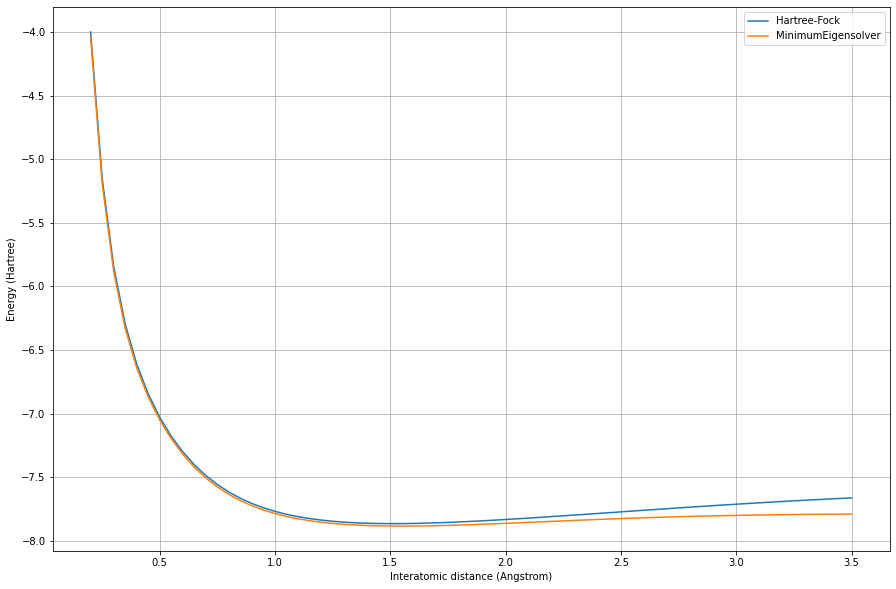
\includegraphics[width=\linewidth]{Images/Capitolo3/Plots/LiH_numpy_minimum_eigensolver_plot.png}
        \caption{NumpyMinimumEigensolver}
    \end{subfigure}
    \hfill
    \begin{subfigure}[h]{0.49\linewidth}
        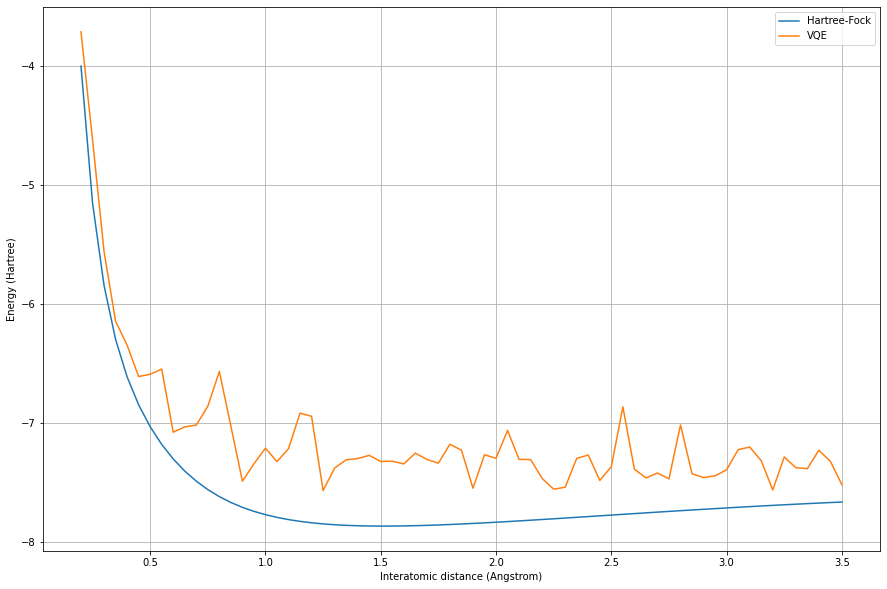
\includegraphics[width=\linewidth]{Images/Capitolo3/Plots/LiH_twolocal_ry_rz_cz_gpu_plot.png}
        \caption{VQE}
    \end{subfigure}%
    \caption[Grafico 7 \newline LiH - TwoLocal - L\_BFGS\_B - Notebook\_GPU - Aer.]{}
    \label{fig:notebookgpu_LiH_aer}
\end{figure}

La sesta simulazione è stata svolta su Notebook\_GPU, con circuito TwoLocal e backend Aer.
I tempi di esecuzione per l'algoritmo VQE si aggirano intorno alle 19 ore e dal grafico di destra si può notare come il risultato non sia per nulla soddisfacente.
%-------------------------------------------------------------------------------------------------------
\subsubsection{Altri ottimizzatori}
L'utilizzo del circuito TwoLocal ci ha permesso di ottenere i risultati migliori, pertanto di seguito verranno mostrate le ultime simulazioni svolte su backend Aer, dove si ricorre ad altri tipi di ottimizzatori.
\newline\newline
\begin{minipage}[b]{0.39\textwidth}
    \scalebox{0.8}{%
    \begin{tabular}[b]{l|c}
        \hline\hline
        \multicolumn{2}{c}{\textbf{\textit{Notebook\_GPU - COBYLA}}}\\
        \hline
        \multirow{3}{*}{\textit{TwoLocal}} & 20:28,53897968928\\
        \cline{2-2} & 20:41,6204098860423\\
        \cline{2-2} & 20:37,403276761373\\
        \hline\hline
    \end{tabular}}
    \captionsetup{type=table}
    \caption[Risultati simulazione COBYLA.]{Nella colonna di destra sono riportati i tempi di esecuzione.}
    \label{table:notebookgpu_cobyla_aer}
\end{minipage}
\hfill
\begin{minipage}[b]{0.57\textwidth}
    \centering
    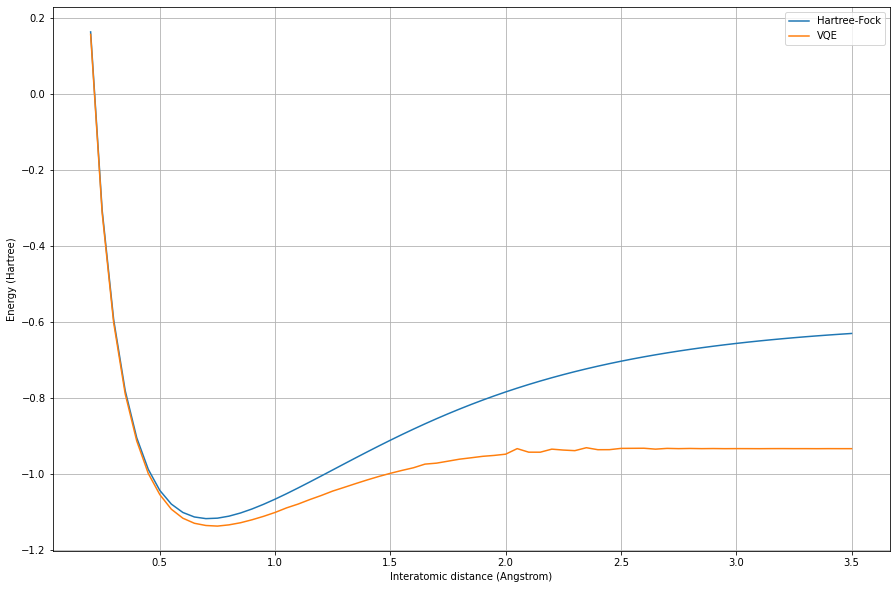
\includegraphics[width=1.0\textwidth]{Images/Capitolo3/Plots/H2_twolocal_ry_rz_cz_cobyla_aer_gpu_plot.png}
    \captionof{figure}[Grafico 8 \newline TwoLocal - COBYLA - Notebook\_GPU - Aer.]{}
    \label{fig:notebookgpu_twolocal_cobyla_aer}
\end{minipage}

I risultati sopra evidenziati (Tabella \ref{table:notebookgpu_cobyla_aer}), inerenti la simulazione svolta su Notebook\_GPU utilizzando il circuito TwoLocal e l'ottimizzatore COBYLA, mostrano dei tempi di esecuzione molto simili ai precedenti. Nel grafico in Figura \ref{fig:notebookgpu_twolocal_cobyla_aer} è possibile vedere delle piccole increspature che non vanno ad incidere notevolmente sull'esito del test.
\newline
\begin{minipage}[b]{0.39\textwidth}
    \scalebox{0.8}{%
    \begin{tabular}[b]{l|c}
        \hline\hline
        \multicolumn{2}{c}{\textbf{\textit{Notebook\_GPU - SPSA}}}\\
        \hline
        \multirow{3}{*}{\textit{TwoLocal}} & 44:13,694082101186\\
        \cline{2-2} & 44:37,829064130783\\
        \cline{2-2} & 46.12,1066045761106\\
        \hline\hline
    \end{tabular}}
    \captionsetup{type=table}
    \caption[Risultati simulazione SPSA.]{Nella colonna di destra sono riportati i tempi di esecuzione.}
    \label{table:notebookgpu_spsa_aer}
\end{minipage}
\hfill
\begin{minipage}[b]{0.57\textwidth}
    \centering
    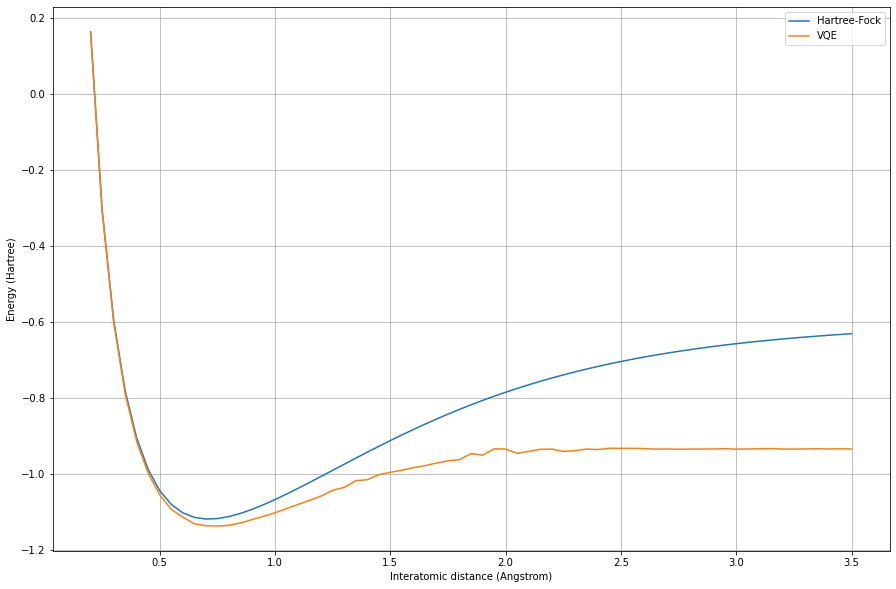
\includegraphics[width=1.0\textwidth]{Images/Capitolo3/Plots/H2_twolocal_ry_rz_cz_spsa_aer_gpu_plot.png}
    \captionof{figure}[Grafico 9 \newline TwoLocal - SPSA - Notebook\_GPU - Aer.]{}
    \label{fig:notebookgpu_twolocal_spsa_aer}
\end{minipage}

Un'ulteriore simulazione è stata fatta utilizzando l'ottimizzatore SPSA.\newline
Come si può vedere nella Tabella \ref{table:notebookgpu_spsa_aer} i tempi di esecuzione risultano raddoppiati ed anche il grafico, mostrato in Figura \ref{fig:notebookgpu_twolocal_spsa_aer}, presenta qualche imperfezione in più.
\begin{figure}[htp]
    \centering
    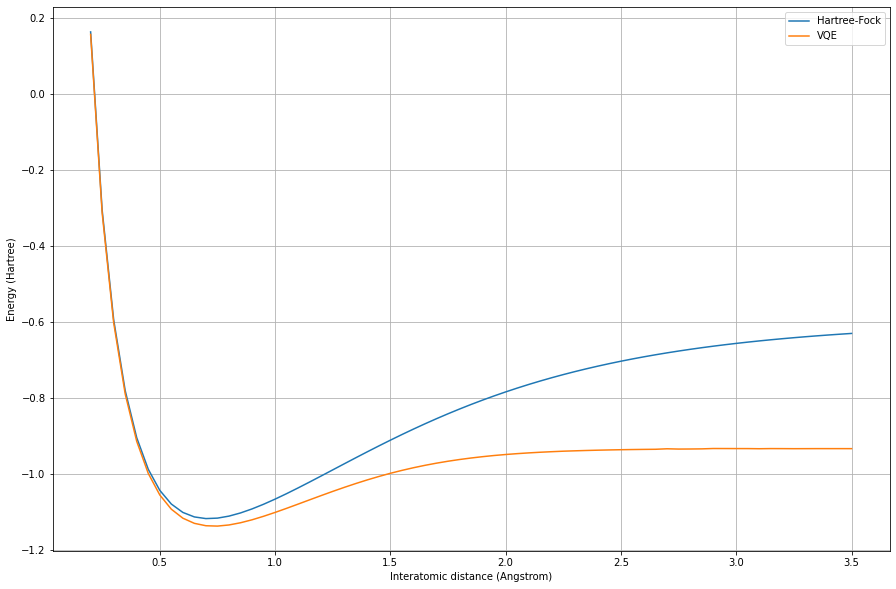
\includegraphics[width=8cm]{Images/Capitolo3/Plots/H2_twolocal_ry_rz_cz_slsqp_aer_gpu_plot.png}
    \caption[Grafico 10 \newline TwoLocal - SLSQP - Notebook\_GPU e Colab\_GPU - Aer.]{}
    \label{fig:notebookgpu_twolocal_slsqp_aer}
\end{figure}
\begin{table}[h]
    \begin{subtable}[h]{0.45\textwidth}
        \centering
        \begin{tabular}[b]{l|c}
            \hline\hline
            \multicolumn{2}{c}{\textbf{\textit{Notebook\_GPU - SLSQP}}}\\
            \hline
            \multirow{3}{*}{\textit{TwoLocal}} & 22:49,5642606417338\\
            \cline{2-2} & 22:51,5691443284354\\
            \cline{2-2} & 21:10,095632870992\\
            \hline\hline
        \end{tabular}
        \caption{}
        \label{table:notebookgpu_slsqp_gpu}
    \end{subtable}
    \hfill
    \begin{subtable}[h]{0.45\textwidth}
        \centering
        \begin{tabular}[b]{l|c}
            \hline\hline
            \multicolumn{2}{c}{\textbf{\textit{Colab\_GPU - SLSQP}}}\\
            \hline
            \multirow{3}{*}{\textit{TwoLocal}} & 26:19,887064695358\\
            \cline{2-2} & 38:01,3527413209276\\
            \cline{2-2} & 26:39,4683996836343\\
            \hline\hline
        \end{tabular}
        \caption{}
        \label{table:colabgpu_slsqp_gpu}
     \end{subtable}
     \caption[Risultati simulazioni SLSQP.]{Nella colonna di destra sono riportati i tempi di esecuzione.}
\end{table}

Come ultimo ottimizzatore è stato utilizzato SLSQP e sono state svolte rispettivamente due simulazioni: la prima riguarda Notebook\_GPU, che è riuscita ad ottenere dei risultati (Tabella \ref{table:notebookgpu_slsqp_gpu}) paragonabili a L\_BFGS\_B con dei tempi di esecuzione molto simili; la seconda riguarda Colab\_GPU, dove i tempi di esecuzione, mostrati nella Tabella \ref{table:colabgpu_slsqp_gpu}, sono di poco superiori.
Uno dei tre test riguardanti questa macchina è stato svolto più volte ma non si è potuto notare un miglioramento.

Entrambe le macchine hanno ottenuto un buon grafico (Figura \ref{fig:notebookgpu_twolocal_slsqp_aer}), molto simile a quello atteso calcolato dall'algoritmo classico NumpyMinimumEigensolver.

%CONCLUSIONI
\chapter*{Conclusioni}
\fancyhead[RO, LE]{\bfseries Conclusioni}
Come si può dedurre dal capitolo precedente, i risultati ottenuti per la molecola d'Idrogeno $H_2$, utilizzando l'algoritmo ibrido VQE, sono tutti tra loro confrontabili.

Attraverso la realizzazione del circuito TwoLocal composto dalle porte logiche quantistiche RY, RZ e CZ, siamo riusciti ad ottenere risultati molto simili a quelli ricavati dall'algoritmo classico NumPyMinimumEigensolver.

I due ottimizzatori che si sono distinti per tempi di esecuzione e bontà del grafico sono stati L\_BFGS\_B e SLSQP: entrambi hanno permesso di effettuare una simulazione in poco più di 20 minuti se consideriamo il backend Aer, più moderno e prestante.

Purtroppo non si è potuto notare un miglioramento utilizzando l'accelerazione hardware della scheda video, pur avendo provato su macchine differenti e teoricamente più performanti.
Questo potrebbe essere causato da qualche metodo di classe all'interno delle librerie Qiskit che ad oggi non riesce ancora probabilmente a gestire correttamente le GPU.

Per quanto riguarda invece la molecola $LiH$, Idruro di Litio, è stato svolto un solo test in quanto, come si è potuto notare, ha impiegato veramente troppo tempo.

Considerando la community di Qiskit molto attiva, sarà probabilmente possibile in futuro eseguire gli stessi esperimenti ottenendo risultati migliori in tempi più brevi, con la possibilità inoltre di effettuare variazioni al codice da noi scritto.
\addcontentsline{toc}{chapter}{Conclusioni}

\newpage 
% BIBLIOGRAFIA
\addcontentsline{toc}{chapter}{Bibliografia}
\fancyhead[RO, LE]{\bfseries Bibliografia}
%\nocite{*}
\bibliographystyle{unsrt}
\bibliography{Bibliografia}

%PAGINA RINGRAZIAMENTI
\chapter*{Ringraziamenti}
\fancyhead[RO, LE]{\bfseries Ringraziamenti}
Ringrazio il Prof. Gervasi per essere sempre stato disponibile ed avermi dato l'opportunità di svolgere questa tesi, facendomi così avvicinare al mondo della computazione quantistica.

Dei sentiti ringraziamenti vanno anche al Dott. Damiano Perri e al Dott. Marco Simonetti, senza i loro preziosi consigli e la loro pazienza non sarei riuscito a portare a termine l'elaborato.

Un grande ringraziamento va alla mia famiglia che mi ha sempre supportato nella mia carriera accademica, agli amici di sempre e a quelli che lo sono diventati nel corso di questi tre anni.

Grazie a tutte le persone che mi sono state vicino aiutandomi a diventare chi sono oggi, inclusi tutti i docenti,
che sono riusciti ad alimentare la passione che ho nei confronti dell'informatica.

% APPENDICE CON IL CODICE SVILUPPATO
\appendix
\linespread{1}
\chapter{Codice}\label{codice:vqe}
\fancyhead[RO, LE]{\bfseries Codice}
Nel paragrafo seguente viene riportato il codice Python necessario per svolgere una simulazione sulla molecola d'Idrogeno.
Verrà utilizzato il circuito TwoLocal in coppia con l'ottimizzatore SLSQP; il backend Aer ci consentirà di specificare la direttiva \textit{statevector\_gpu} per l'utilizzo della scheda video.

\section{H2 - TwoLocal - SLSQP - Aer - GPU}
\begin{footnotesize}
\begin{minted}[linenos=tru]{python}
from time import time

import matplotlib.pyplot as plt
import numpy as np

from qiskit import Aer
from qiskit.aqua import aqua_globals, QuantumInstance
from qiskit.aqua.algorithms import NumPyMinimumEigensolver, VQE
from qiskit.aqua.components.optimizers import SLSQP
from qiskit.circuit.library import TwoLocal
from qiskit.chemistry.drivers import PySCFDriver, UnitsType
from qiskit.chemistry.core import Hamiltonian, QubitMappingType

start = 0.2
step = 0.05
end = 3.5
d = np.arange(start, end + step, step)
molecule = "H .0 .0 .0; H .0 .0 {0}"
energies = np.zeros(d.size)
hf_energies = np.zeros_like(energies)
distances = np.zeros_like(energies)

# NumPyMinimumEigensolver
for i, v in enumerate(d):
    driver = PySCFDriver(atom=molecule.format(v),
    unit=UnitsType.ANGSTROM,
    basis='sto3g')
    
    qmolecule = driver.run()
    operator = Hamiltonian(qubit_mapping=QubitMappingType.PARITY,
                           two_qubit_reduction=False)
    qubit_op, aux_ops = operator.run(qmolecule)
    result = NumPyMinimumEigensolver(qubit_op).run()
    result = operator.process_algorithm_result(result)
    energies[i] += result.energy
    hf_energies[i] += result.hartree_fock_energy
    distances[i] += v
    
print('Distances: ', distances)
print('Energies:', energies)
print('Hartree-Fock energies:', hf_energies)

plt.figure(figsize=(15,10))
plt.plot(distances, hf_energies,
label="Hartree-Fock")
plt.plot(distances, energies,
label="MinimumEigensolver")

plt.xlabel("Interatomic distance (Angstrom)")
plt.ylabel("Energy (Hartree)")
plt.legend()
plt.grid()

# VQE
aqua_globals.random_seed = 50

energies = np.zeros(d.size)
hf_energies = np.zeros_like(energies)
distances = np.zeros_like(energies)

qi = QuantumInstance(Aer.get_backend('statevector_simulator'),
                    backend_options={"method":"statevector_gpu"},
                    seed_simulator=aqua_globals.random_seed,
                    seed_transpiler=aqua_globals.random_seed)

start_time = time()
for i, v in enumerate(d):
    driver = PySCFDriver(atom=molecule.format(v),
                        unit=UnitsType.ANGSTROM,
                        basis='sto3g')
    
    qmolecule = driver.run()
    operator = Hamiltonian(qubit_mapping=QubitMappingType.PARITY,
                           two_qubit_reduction=False)
    qubit_op, aux_ops = operator.run(qmolecule)
    optimizer = SLSQP(maxiter=250)
    var_form = TwoLocal(qubit_op.num_qubits, ['ry', 'rz'],
                        'cz', reps=5)
    algo = VQE(qubit_op, var_form, optimizer)
    result = algo.run(qi)
    result = operator.process_algorithm_result(result)
    energies[i] += result.energy
    hf_energies[i] += result.hartree_fock_energy
    distances[i] += v

execution_time = (time() - start_time)

print('Distances: ', distances)
print('Energies:', energies)
print('Hartree-Fock energies:', hf_energies)
print('Execution time (minutes):', (execution_time/60))

var_form.draw(output="mpl")

plt.figure(figsize=(15,10))
plt.plot(distances, hf_energies,
label="Hartree-Fock")
plt.plot(distances, energies,
label="VQE")

plt.xlabel("Interatomic distance (Angstrom)")
plt.ylabel("Energy (Hartree)")
plt.legend()
plt.grid()

# Python 3.8.5
# Qiskit version
import qiskit
print(qiskit.__qiskit_version__)

'''
{'qiskit-terra': '0.15.2',
 'qiskit-aer-gpu': '0.6.1',
 'qiskit-ignis': '0.4.0',
 'qiskit-ibmq-provider': '0.10.0',
 'qiskit-aqua': '0.7.5',
 'qiskit': '0.22.0'}
'''
\end{minted}
\end{footnotesize}


\chapter{Glossario}
\fancyhead[RO, LE]{\bfseries Glossario}

Spiegazione di alcune sigle utilizzate nei vari capitoli.
\newline
Fonti:
\begin{verbatim}
https://en.wikipedia.org/wiki/
https://docs.conda.io/en/latest/
https://docs.microsoft.com/
\end{verbatim}

\textbf{\textit{EPR}}: The Einstein–Podolsky–Rosen paradox (EPR paradox) is a thought experiment proposed by physicists Albert Einstein, Boris Podolsky and Nathan Rosen (EPR), with which they argued that the description of physical reality provided by quantum mechanics was incomplete. In a 1935 paper titled "Can Quantum-Mechanical Description of Physical Reality be Considered Complete?", they argued for the existence of "elements of reality" that were not part of quantum theory, and speculated that it should be possible to construct a theory containing them. Resolutions of the paradox have important implications for the interpretation of quantum mechanics.

\textbf{\textit{API}}: An application programming interface is a computing interface which defines interactions between multiple software intermediaries. It defines the kinds of calls or requests that can be made, how to make them, the data formats that should be used, the conventions to follow, etc. It can also provide extension mechanisms so that users can extend existing functionality in various ways and to varying degrees.

\textbf{\textit{Conda}}: Conda is an open source package management system and environment management system that runs on Windows, macOS and Linux. Conda quickly installs, runs and updates packages and their dependencies. Conda easily creates, saves, loads and switches between environments on your local computer. It was created for Python programs, but it can package and distribute software for any language.

\textbf{\textit{WSL2}}: The Windows Subsystem for Linux lets developers run a GNU/Linux environment -- including most command-line tools, utilities, and applications -- directly on Windows, unmodified, without the overhead of a traditional virtual machine or dualboot setup.
\newline\newline
Spiegazione di alcuni ottimizzatori utilizzati nella fase sperimentale.
\newline
Fonte: documentazione di Qiskit, reperibile al seguente indirizzo
\begin{verbatim}
https://qiskit.org/documentation.
\end{verbatim}

\textbf{\textit{COBYLA}}: Constrained Optimization By Linear Approximation optimizer. COBYLA is a numerical optimization method for constrained problems where the derivative of the objective function is not known.

\textbf{\textit{SPSA}}: Simultaneous Perturbation Stochastic Approximation (SPSA) optimizer. SPSA is an algorithmic method for optimizing systems with multiple unknown parameters. As an optimization method, it is appropriately suited to large-scale population models, adaptive modeling, and simulation optimization. SPSA is a descent method capable of finding global minima, sharing this property with other methods as simulated annealing. Its main feature is the gradient approximation, which requires only two measurements of the objective function, regardless of the dimension of the optimization problem.

\textbf{\textit{SLSQP}}: Sequential Least SQuares Programming optimizer. SLSQP minimizes a function of several variables with any combination of bounds, equality and inequality constraints. The method wraps the SLSQP Optimization subroutine originally implemented by Dieter Kraft. SLSQP is ideal for mathematical problems for which the objective function and the constraints are twice continuously differentiable. Note that the wrapper handles infinite values in bounds by converting them into large floating values.

\chapter{Link delle figure}
\fancyhead[RO, LE]{\bfseries Link delle figure}

\small
\sloppy
\section{Capitolo 1}
\begin{itemize}
    \renewcommand\labelitemi{--}
    \item \url{https://turingmachine.io/}
\end{itemize}

\section{Capitolo 2}
\begin{itemize}
    \renewcommand\labelitemi{--}
    \item \url{https://fstechadvisory.accenture.com/wp-content/uploads/2018/03/Fig.-1.1-Qubit-superposition.jpg}
    
    \item \url{https://i.stack.imgur.com/GQxa8.png}

    \item \url{http://mondodigitale.aicanet.net/2013-4/articoli/01\_Computer\_Quantistici.pdf}

    \item \url{https://encrypted-tbn0.gstatic.com/images?q=tbn\%3AANd9GcScBdRbfD77h9KvkdoxnK5ndtlqISyiIhTZVQ\&usqp=CAU}

    \item \url{https://doi.org/10.1021/acs.chemrev.8b00803}
    
    \item \url{https://encrypted-tbn0.gstatic.com/images?q=tbn\%3AANd9GcTz_RM2pKJ-UkxWFjnNBtUMga6LVUDSy111dQ\&usqp=CAU}
    
    \item \url{https://www.giuseppesottile.it/articles/graphic/qubit.png}
    
    \item \url{https://miro.medium.com/max/1450/1*upoirxvOvNalDN7l0TWFQg.png}
    
    \item \url{https://encrypted-tbn0.gstatic.com/images?q=tbn\%3AANd9GcT1h7LdYuFEE0ksGO_GXYTUJ1EwzA7VZi5j8A\&usqp=CAU}
\end{itemize}

\section{Capitolo 3}
\begin{itemize}
    \renewcommand\labelitemi{--}
    \item \url{https://qiskit.org/documentation/_images/qiskit-framework.png}
\end{itemize}

\end{document}